% REMEMBER: You must not plagiarise anything in your report. Be extremely careful.

\documentclass[british,table,svgnames,xcdraw]{l4proj}

%
% put any additional packages here
%
\usepackage{csquotes}
\usepackage{multirow}
\usepackage{tabularx}

\usepackage{isodate}
\usepackage{inconsolata}
\usepackage{bbm}

\usepackage{jfdm-plt}
\usepackage{mylang}
\usepackage{url}
\usepackage{cleveref}

\usepackage[acronym,toc]{glossaries}

\renewcommand{\abstitlestyle}[1]{{{\let\newpage\relax\chapter*{#1}\thispagestyle{empty}}}}

% let us define a definition for unnumbered chapters.
\titleformat{name=\chapter,numberless}
            [display]
            {\normalfont\huge\bfseries\secfont}
            {}
            {0pt}
            {}

\makenoidxglossaries

\newacronym{dcs}{SoCS}{School of Computing Science}
\newacronym{abe}{ABE}{Attribute Based Encryption}
\newacronym{mks}{MKS}{Master Key Server}
\newacronym{prs}{PRS}{Public Resource Server}
\newacronym{crs}{CRS}{Client Resource Server}
\newacronym{aes}{AES}{Advanced Encryption Standard}
\newacronym{uuid}{UUID}{Universally Unique IDentifier}
\newacronym{rbac}{RBAC}{Role Based Access Control}
\newacronym{abac}{ABAC}{Attribute Based Access Control}
\newacronym{xacml}{XACML}{eXtensible Access Control Markup Language}
\newacronym{pep}{PEP}{Policy Enforcement Point}
\newacronym{pdp}{PDP}{Policy Decision Point}
\newacronym{jwt}{JWT}{JSON Web Token}
\newacronym{html}{HTML}{Hypertext Markup Language}
\newacronym{tls}{TLS}{Transport Layer Security}
\newacronym{ssl}{SSL}{Secure Sockets Layer}
\newacronym{ca}{CA}{Certificate Authority}
\newacronym{gui}{GUI}{Graphical User Interface}
\newacronym{cli}{CLI}{Command Line Interface}
\newacronym{os}{OS}{Operating System}
\newacronym{hsm}{HSM}{Hardware Security Module}

\begin{document}

%==============================================================================
%% METADATA
\title{A Cryptographically Secure Departmental Resource Server}
\author{Christopher Watson}
\date{March 7, 2019}

\maketitle

\newcommand{\thePolicyLang}{\textsc{PolLang}\textsubscript{ABE}\xspace}
\newcommand{\theResServer}{\textsc{ResSrvr}\textsubscript{ABE}\xspace}
\newcommand{\OpenABE}{\textsc{OpenABE}\xspace}
\newcommand{\PyOpenABE}{\textsc{PyOpenABE}\xspace}

%==============================================================================
%% ABSTRACT
\begin{abstract}
  Development of a cryptographically secure resource server for staff \& students of the Department of Computing Science to distribute encrypted resources internally.\\
  Resources can be encrypted with unique, fine-grained policies of attributes that must then be resolved by an end user's private key in order to complete decryption.
  \vskip 0.5em
  Required the implementation and deployment of an Attribute-Based Encryption system built from a cryptographically-proven external library and designed with a complete enrolment process for generating \& signing user private keys securely.\\
  Requirements are proven by cryptographic mathematics, use-case based testing and a risk assessment of the system's deployment according to ISO 27005.
\end{abstract}


%==============================================================================

% EDUCATION REUSE CONSENT FORM
% If you consent to your project being shown to future students for educational purposes
% then insert your name and the date below to  sign the education use form that appears in the front of the document.
% You must explicitly give consent if you wish to do so.
% If you sign, your project may be included in the Hall of Fame if it scores particularly highly.
%
% Please note that you are under no obligation to sign
% this declaration, but doing so would help future students.
%
\def\consentname {Christopher Watson} % your full name
\def\consentdate {31 January 2019} % the date you agree
%
\educationalconsent


%==============================================================================
\tableofcontents

%==============================================================================
%% Notes on formatting
%==============================================================================
% The first page, abstract and table of contents are numbered using Roman numerals and are not
% included in the page count.
%
% From now on pages are numbered
% using Arabic numerals. Therefore, immediately after the first call to \chapter we need the call
% \pagenumbering{arabic} and this should be called once only in the document.
%
% The first Chapter should then be on page 1. You are allowed 40 pages for a 40 credit project and 20 pages for a
% 20 credit report. This includes everything numbered in Arabic numerals (excluding front matter) up
% to but excluding the appendices and bibliography.
%
% You must not alter text size (it is currently 10pt) or alter margins or spacing.
%
%
%==================================================================================================================================
%
% IMPORTANT
% The chapter headings here are **suggestions**. You don't have to follow this model if
% it doesn't fit your project. Every project should have an introduction and conclusion,
% however.
%
%==================================================================================================================================

\chapter{Introduction}
\label{ch:introduction}

% reset page numbering. Don't remove this!
\pagenumbering{arabic}

%==============================================================================
%% INTRODUCTION

Sharing resources securely across organisations or departments is both a difficult and daunting task, with common methods relying on forms of Role-based access control (RBAC) to grant access to, often unencrypted, resource buckets. However these methods are unable to provide a fine-grained system for either precise or modular access and cannot protect the resources should the system become compromised.\\
Clearly, a level of granularity is required in order to configure appropriate access restrictions to resources and provide long-term support for the system through dynamic access control. RBAC is also complex to configure properly and due to the nature of roles, can risk accidental access grants through roles that are too expansive in permissions.\\
These problems can be solved with the use of an Attribute-Based Encryption (ABE) system which improves security by handling the advanced encryption of resources through a defined policy language which allows for unique, granular access to resources on a per-user basis.\\
Unlike RBAC, an ABE system utilises a policy language to create bespoke, per-resource attribute policies that define specific access restrictions for the resource they are embedded into. This means that a user can only decrypt a resource if they can cryptographically prove assignment of the required attributes in their private keys - generated \& signed by a central master key server.

\section{Overview}
\label{sec:intro_overview}

This project aimed to develop a full resource server product that meets the definition of "cryptographically secure"; where resources are encrypted at rest and only transmitted \& stored in a secure, unreadable ciphertext format. Thus, the system would never be aware of the contents of the resources stored and implicitly, the resources will remain secure even in the event of the system becoming compromised. The product as a whole was determined to need 2 servers:
\begin{enumerate}
  \item an offline 'cold storage' master key server to generate user keys
  \item an online 'dumb' resource server to store and manage the ABE encrypted resources
\end{enumerate}
Due to the utilisation of ABE, communication with the resource server is too complex and verbose for a standard user and as such, a tool is provided for users that simplifies interactions. Subsequently, a user can choose to run a simple local web client for this communication with the resource server, providing the following services:
\begin{enumerate}
  \item downloading of encrypted resources
  \item decryption of encrypted resources
  \item encryption of unencrypted resources
  \item uploading of encrypted resources
  \item searching for uploaded resources
  \item determining policies of uploaded resources
  \item creating a policy for a new resource
\end{enumerate}
All these services are then accessible through a basic GUI that aims to obscure the complexity of ABE from the user; reducing the learning curve to use of the product.


\section{Aims}
\label{sec:intro_aims}

The main aim of the project was to produce an end product that can serve as a cryptographically secure resource server for a department and its users, with a configurable and dynamic system for access control.
Production of the service required careful research and design before implementation to determine both the end users of the service and the needs of the department. To achieve this, the project aimed to identify the users in the scenario of the \acrfull{dcs} with an analysis of the structure of staff and students.
\vskip 0.5em
The project needed to consider the enrolment process of bringing new users into the system and create a valid procedure for creating cryptographic keys for users. This includes determining the validity of a user's attributes and identifying an authority that can securely be tasked with performing said validation.
The service would have to implement and show the security of an \acrfull{abe} system with real-world use cases to prove its effectiveness in the scope of securely distributing resources amongst members of a department. Further, the system would also have to undergo a risk assessment to determine the actual security of the system whilst identifying risk factors within the service.
\vskip 0.5em
It was determined that creating an \acrshort{abe} library was beyond the project scope, so the project identified and then integrated the external \OpenABE library (described in \Cref{sec:bkgr_openabe}). Determination of which \acrshort{abe} library focused on the extensibility of the library as well as evidence of the library in use for a similar scenario as a departmental resource server.
The project looked into the Johns Hopkins Hospital deployment of an electronic medical records system, \citet{Akinyele2011}. This represented a good scenario for comparison, as the secure distribution of medical records amongst staff and patients relied on dynamic and extremely granular access control but with an even higher requirement for security than that of a departmental resource server.
\vskip 0.5em
Deployment scenarios were sufficiently similar such that the setup used for the Johns Hopkins deployment would, in fact, have translated well to the project's deployment scenario, including the enrolment process (by which a user receives their private key from a central admin service) and the granularity of the policies used to encrypt records.

However, the Johns Hopkins team required the use of mobile applications as end devices and also the ability to update the user's private key remotely. Both features were determined to be very high risk and ultimately unnecessary for the scope of the \theResServer system. Additionally, the Johns Hopkins deployment relied on all new data coming from one source \textemdash\ the hospital \textemdash\ and so was built on the basis that one system would be able to encrypt all records. A resource server however, must be able to receive resources from many different sources and in the project's case, any member of the \acrshort{dcs} would need to be able to encrypt \& decrypt resources locally.


\section{Contributions}
\label{sec:intro_contrib}

\subsection{Policy Language}
\label{subsec:intro_pol_lang}

The project produced a formal language definition of a policy language for the ABE system, known as \thePolicyLang. This language, allows the ABE system to clearly define the structure of all policies, ensuring reliable and consistent use over all resources.\\
The \thePolicyLang definition includes the syntax and types, along with the typing rules that are enforced on a policy before encryption of a resource can be processed. The definition also includes substitution rules and the required big step semantics for the language, with a final interpretation definition to interpret \thePolicyLang to the Python bindings used in the product.

\subsection{Software}
\label{subsec:intro_software}

Production of the resource service required the defining of two servers (as described above) and the creation of the services running on each. Additionally, a third product was created to ease use of the service for users, in the form of a local web GUI client that handles communication with the resource service for the user.
\vskip 0.5em
An offline master key server would be tasked with initiating the ABE system and provisioning the master private key for the entire service. This server would remain offline from the point of complete installation, ensuring that the key is provisioned after the server enters the offline state and protecting the master private key from external threats.\\
A separate online, 'dumb' storage service for all encrypted resources, would only ever store the ciphertext binary blobs with no method of decrypting or reading any uploaded resources. This storage service would also be responsible for distributing the master public key, which could be manually uploaded from the master key server using a physical, offline transfer.\\
An end user product can be ran locally on a user's device and then connected to the storage service to provide the services on offer through a simple GUI\@. The user could then provide this local client with their private user key and the service would use it to \textit{locally} decrypt any resources, ensuring the key never leaves the user's device. For encrypting, the local client retrieves the master public key from the resource server and performs encryption on any required resources using the public key and the relevant policies, as defined by the user.


\section{Outline}
\label{sec:intro_outline}

\begin{enumerate}
  \item \textbf{Background}
  \begin{enumerate}
    \item Access control \& encryption
		\item Public key infrastructure \& resource servers
		\item \OpenABE library and \PyOpenABE bindings
  \end{enumerate}
  \item \textbf{Analysis/Requirements}
  \begin{enumerate}
    \item Security considerations
    \item Deployment requirements
    \item Requirements for enrolling
		\item Case Studies for deployment scenario
  \end{enumerate}
	\item \textbf{Design}
  \begin{enumerate}
    \item Design of the \thePolicyLang language
    \item Signing \& using user keys
    \item Deployment scenario \& system architecture
		\item Building policies \& searching across filenames
  \end{enumerate}
	\item \textbf{Implementation}
  \begin{enumerate}
    \item Working with the \OpenABE toolset
    \item Choosing Python's Flask for web servers
    \item Client server security
		\item Storing data with mongoDB
		\item Fuzzy string matching for filenames
  \end{enumerate}
	\item \textbf{Evaluation}
  \begin{enumerate}
    \item Security evaluation \& risk assessment
    \item Successfully achieved
    \item Failed to achieve
  \end{enumerate}
	\item \textbf{Conclusion}
  \begin{enumerate}
    \item Summary of project
    \item Future work
    \item Problems tackled during project
		\item Real-world deployment
  \end{enumerate}
\end{enumerate}


%==================================================================================================================================
\chapter{Background}
\label{ch:background}

We present background information for the project, with discussion of Access Control systems and Encryption methods, as well as the concept of Public Key Infrastructures. We further present the uses \& requirements of Resource Servers, along with identifying an \acrshort{abe} tool for the system; the \OpenABE library.

\section{Access Control}
\label{sec:bkgr_acc_ctrl}

Access Control encompasses the authentication and authorisation of users in a system, as well as the audit process for said system. In the scope of this project, we only consider the authorisation part of Access Control, since the service does not authenticate users before permitting the upload or download of resources, because the encryption of resources protects against rogue access of data. The Design chapter (\cref{ch:design}) discusses this decision further, but since users are not authenticated by the \acrfull{prs}, it is also difficult to audit the service due to lack of information on users.

\subsection{RBAC \& ABAC}
\label{subsec:acc_ctrl_rbac_abac}

Access Control is vital to maintaining the security of online services as it allows users to be granted access to certain routes, documents and data, but denied access to others. This most often takes the form of \acrfull{rbac} \citep{Sandhu1996}, where users are assigned a role such as `\textit{Customer}', `\textit{Staff}' or `\textit{Admin}' with each role having a different set of permissions.

For example, a user with the `\textit{Customer}' role would not have access to the organisation's internal documents, whereas a user with the `\textit{Staff}' role would. Similarly, a user with the `\textit{Staff}' role would not necessarily have access to a service's user details, whereas a user with the `\textit{Admin}' role would.

Some \acrshort{rbac} systems can grant a user multiple roles with different permissions, although it is also possible to have each role set up to grant a subset of the permissions granted by another role. For example, a `\textit{Superadmin}' role would have all permissions, with a lower `\textit{Admin}' role having a subset of those permissions; such as not having permission to edit or delete other `\textit{Admin}' accounts.
\vskip 0.5em
A more advanced form of Access Control exists in \acrfull{abac} \citep{Hu2014}, where users are assigned attributes that describe them as an individual. Policies can then be created that dictate the attributes required to access a resource or route for a system. The standard for \acrshort{abac} is the \acrfull{xacml} \citep{Parducci2010}.

In \acrshort{abac}, a user might be granted attributes such as \texttt{`role:customer, dob:02/06/1992, username:johnsmith, email:john@example.com, city:Glasgow'} and attempt to access a resource with a policy such as \texttt{`role==customer and city==Edinburgh and dob<=01/01/2003'}. The user would not be granted access in this case, as they are from \textit{Glasgow} and not \textit{Edinburgh}, despite being a \textit{customer} born before \textit{January 1, 2003}. This offers a level of granularity that \acrshort{rbac} cannot match.
\vskip 0.5em
Both \acrshort{rbac} and \acrshort{abac} are implemented through assigning requirements to different routes or resources that are then enforced through interceptions of requests by users. When a user makes a request to the service, it is intercepted by a \acrfull{pep} that gathers the user's details from the request and submits an authorisation request to a \acrfull{pdp}.

The \acrshort{pdp} then verifies if the user has the correct permissions to access the resource. If using a \acrshort{rbac} system, the \acrshort{pdp} checks if the role the user has is privileged enough to be granted access. If using an \acrshort{abac} system, the \acrshort{pdp} checks that the user's attributes can be resolved by the policy assigned to the resource, before then granting access if the policy has resolved to true.

In both scenarios the \acrshort{pep} may have retrieved a session from the user's request and then the \acrshort{pdp} would have retrieved their details from an authentication system or session storage.

\subsection{Models}
\label{subsec:acc_ctrl_models}

Other Access Control models do exist and generally all models fall into one of two categories, \textbf{capability-based} models or \textbf{access control lists-based} (ACL-based) models; where \acrshort{rbac} represents a capability-based model and \acrshort{abac} represents an ACL-based model.
\vskip 0.5em
\textit{Capability-based models} are based on the ability of a user to prove possession of an unforgeable reference or \textit{capability} that aligns with the references of the system they are authorising against. In the case of \acrshort{rbac}, the user proves that they have the \textit{role} required for access via some immutable piece of data such as a cookie or \acrfull{jwt} (described in RFC 7519 \citep{Jones2015}).

\textit{ACL-based models} are instead based around a user's identity appearing in a list assigned to or embedded within the object, data or route they are attempting to access. In the case of \acrshort{abac}, a policy is attached to a route or resource served by the service the user is attempting to access. The policy serves as the role of the list and a user's attributes are embedded in a cookie or \acrshort{jwt} which identity the user and must then be parsed by the policy.

\subsection{Representing ABAC Policies}
\label{subsec:acc_ctrl_abac_policies}

Although \acrshort{xacml} is the standard for writing and enforcing \acrfull{abac} policies, the format is verbose and difficult to interpret. We therefore suggest an alternative format for describing policies within this report.

We define two entities, \textbf{\textit{Subject} s} and \textbf{\textit{Environment} e}, such that \textbf{s} represents the subject attempting to access a resource (\textit{the user}) and has been assigned their respective attributes, and \textbf{\textit{Environment} e} represents the environment the subject is within and has implicit attributes that relate to said environment, such as locale, location \& datetime.
\vskip 0.5em
We then define the attributes that both \textbf{\textit{Subject} s} and \textbf{\textit{Environment} e} have in relation to the \acrshort{abac} policy:
\begin{itemize}
  \item[]
    \textbf{s} $\Rightarrow$ role, jobField, studentLevel, enrolledCourses
  \item[]
    \textbf{e} $\Rightarrow$ currentDate, location
\end{itemize}
\vskip 0.5em
From the fully defined \textbf{\textit{Subject} s} and \textbf{\textit{Environment} e} entities, we can then produce an example access policy as shown in \cref{fig:bkgr_abac_policy} using each entity's attributes and set values to restrict access. In this case, we define a policy for a resource that can only be accessed by a staff member in the \textit{Research \& Teaching} field. Alternatively, the policy also allows for a Level 2 student that has enrolled in the four courses, \textit{2001, 2005, 2011 \& 2018}, but only if the current date is beyond the arbitrary release date of \textit{27 March 2019} and the student is located in \textit{Glasgow, UK}.

\begin{figure}[ht]
  \centering
\begin{align*}
  \text{Policy(\textbf{s},\textbf{e})}
  &
    \leftarrow
    \text{( role(\textbf{s})} \equiv \text{`Staff'}
  \\
  &
    \phantom{::::::::}\wedge
    \text{jobField(\textbf{s})} \equiv \text{`Research \& Teaching' )}
  \\
  &
    \phantom{::}\vee
    \text{( role(\textbf{s})} \equiv \text{`Student'}
  \\
  &
    \phantom{::::::::}\wedge
    \text{studentLevel(\textbf{s})} \equiv \text{2}
  \\
  &
    \phantom{::::::::}\wedge
    \text{enrolledCourses(\textbf{s})} \equiv \text{[2001, 2005, 2011, 2018]}
  \\
  &
    \phantom{::::::::}\wedge
    \text{currentDate(\textbf{e})} \geq \text{27 March 2019 }
  \\
  &
    \phantom{::::::::}\wedge
    \text{location(\textbf{e})} \geq \text{Glasgow, UK )}
\end{align*}
  \caption{
    \label{fig:bkgr_abac_policy}
    An example \acrshort{abac} policy dictating access to a resource.
    Successful decryption would be possible for a member of staff in the Research \& Teaching field \textbf{or} a Level 2 student enrolled in the 2001, 2005, 2011 \& 2018 courses if the lecture slides' release date has passed and the location of the student is Glasgow, UK.
  }
\end{figure}


\section{Encryption}
\label{sec:bkgr_encryption}

Encryption is the process of encoding information in a manner such that only authorised parties can later decode and access the encoded information, known as decrypting. Non-authorised parties can complete decryption successfully and as such an encrypted piece of information stays secret in transit and storage, until decrypted by an authorised party.

An encrypted resource, such as an encrypted PDF, is best understood as an unintelligible scramble of data which cannot be understood directly by either computer or user \citep{Heys1994}. Only upon a successful decryption operation can the information be retrieved again, where such an operation returns the original information now back in its decrypted form that can then be processed by any party again.
\vskip 0.5em
At the basic level, encryption can be categorised as \textit{symmetric} or \textit{asymmetric}, referring to either having a single pre-shared key used for all encryption \& decryption \citep{Massey1988} or having per-party key-pairs with each party holding a public \& private key for communication \citep{Diffie1976}. Thus the single pre-shared key setup is considered to be \textit{symmetric} and the alternative is considered \textit{asymmetric} due to the different keys for each party.

The background for the project only considers \textit{asymmetric} setups due to the difficulty of securely distributing pre-shared keys and as such breaks down the differences in \textbf{1-to-1} \& \textbf{1-to-Many} asymmetric encryption implementations.

\subsection{1-to-1 Encryption}
\label{subsec:bkgr_enc_1to1}

Classical encryption relates to a 1-to-1 relationship whereby one party encrypts information for a single other party, such that only that other party may decrypt the data. This scenario is perfect for when one party wishes to send a resource to only the other party, such as securely sending legal documents to a lawyer. This 1-to-1 method of encryption also remains the most prevalent form, in part due to its use in the \acrfull{tls} standard for web communication \citep{Rescorla2018}, where it helps to secure communication between a web browser and the web server a user is accessing.

Implementations of 1-to-1 encryption rely on the provisioning of key pairs \citep{Diffie1976}, where each party creates a private and public key for themselves. Each party then publishes their public key to the other party and keep their private key secret.
\vskip 0.5em
Communication can then take place between the two parties by a system where party A encrypts a message or document for party B, by signing said message with party B's public key. \citet{Gaithuru2015} describes how this then allows only party B to decrypt the message \textemdash\ by using their secret private key \textemdash\ ensuring that only party B is able to interpret the sent message and that for party B to then securely respond to party A, they must encrypt their response by signing the desired information with the public key of party A.

This ensures secure information transmission between the two parties and also guarantees that any data sent between the two parties can be safely deposited on unprotected storage without risk of the information being extracted through decryption. Unfortunately, despite the high security, 1-to-1 encryption cannot work for a resource server since multiple users must be able to access a single resource and storing \textit{n} copies of a resource \textemdash\ individually encrypted for each user \textemdash\ is unmanageable.

\subsection{1-to-Many Encryption}
\label{subsec:bkgr_enc_1toM}

A more modern approach to encryption is rapidly growing in adoption across the industry, as the need for secure communication between multiple parties continues to increase \citep{Berger2016}. Examples of such scenarios include secure messaging applications such as WhatsApp, conference video calls between multiple users and company-wide, internal memos or resources.

Different scenarios achieve secure 1-to-Many encryption by different means, as the method must match the desired scenario properly. A balance must be struck between security, speed and efficiency in order for a product to offer the services its users require.
\vskip 0.5em
Implementations of 1-to-Many encryption cannot rely on simple, per-party key pairs in the same manner that 1-to-1 manages. This is because in order for many parties to communicate together, each party must store the public key of \textbf{every} other party and then encrypt any information they wish to send \textit{many} times; encrypting the information with each other party's public key in turn.

When the number of parties is limited, this is both fast and manageable for most systems, however issues arise when \textit{1000s} or even \textit{10000s} of parties wish to communicate. Further, adding and removing parties from the communication results in updates for all other parties, whilst revocation of access can be complex and inefficient.
\vskip 0.5em
Products such as WhatsApp and other chatrooms or messaging services, often implement a method wherein a single key is required for both encrypting \& decrypting messages \citep{Rosler2018}. This is a form of \textit{symmetric} encryption, however the pre-shared key is first shared between all parties by using \textit{asymmetric} public keys for each party from a central server or original party.

Solutions such as \acrfull{abe} provide an alternative that does not require participating parties to know other party keys or for the sending party to know all parties that they are communicating with. This also limits the effects of removing parties from communication and offers seamless adding of new parties, since in both cases an update need not be provided to the other parties.

\subsection{Attribute Based Encryption}
\label{subsec:bkgr_enc_abe}

\acrfull{abe} is an encryption method which aims to offer the same capabilities as \acrshort{abac} (\Cref{subsec:acc_ctrl_rbac_abac}) but applied directly to the encryption \& decryption of resources. This allows attributes and policies to directly be embedded into encrypted resources and \acrshort{abe} implements two schemes of encryption, the key-policy scheme and the ciphertext-policy scheme \citep{Waters2011}.
\vskip 0.5em
Using the key-policy scheme requires defining a user's access to resources in their user key in the form of a policy such as \textit{`access to all algorithmics course resources for the 2018\textemdash2019 academic year'}, with attributes assigned to resources and embedded into their ciphertexts. Access to the resource is then granted only if the resources meet the policy defined by the user's key.

The ciphertext-policy scheme is the polar opposite in implementation, where instead a resource ciphertext has the embedded policy and the users' keys have attributes describing the user. A ciphertext in this scenario, might have a policy such as \textit{`access if user is a student in the Networking course or user is a member of staff'} and access would be granted to a user if and only if their key has the required attributes.
\vskip 0.5em
The process \acrshort{abe} requires to encrypt \& decrypt resources is analysed and described in \Cref{subsec:analysis_abe}, including its use of both \textit{symmetric} and \textit{asymmetric} encryption.


\section{Public Key Infrastructure}
\label{sec:bkgr_pub_key_infr}

Public key cryptography is briefly discussed in the \nameref{sec:bkgr_encryption} section above and is originally attributed to \citet{Diffie1976} where a full description of the pubic key encryption \& decryption processes can be found.\\
When employed in a real-world product, public key cryptography requires an infrastructure for the distribution of public keys. This is an absolute requirement, as an end user must be able to trust that the public key they have received is genuinely the public key of the system or person they are communicating with.\\
Chatrooms or messaging services have central servers that process this distribution of public keys, ensuring that any party of the communication may verify public keys against a single authority. If a public key fails verification with that authority, then a user may assume that the public key they have received is a rogue or otherwise invalid key.
\vskip 0.5em
In the case of websites and the \acrshort{tls} protocol \citep{Rescorla2018}, each server hosting a website must communicate with a browser via the \acrshort{tls} protocol, verifying the communication with a \acrshort{tls}/\acrshort{ssl} certificate. The browser requires the ability to then validate that a certificate it has received, does indeed belong to the website they are trying to visit. Hence, Certificate Authorities (\acrshort{ca}s) serve this purpose for the Internet, by validating that a served certificate is genuinely from the website it claims to be.\\
In the case of the Internet, \acrshort{ca}s are independent, pre-approved companies that securely authorise that a server is genuinely owned and operated by/for a website with tools such as DNS validation \citep{Hunt2001}. These \acrshort{ca}s are thus the full and final authorisation that a browser is genuinely communicating securely with the website the user intended to visit.
\vskip 0.5em
A deployed resource server system must also be able to process the verification of its distributed public key or risk users encrypting resources with a rogue key. Whilst such a deployment would make use of \acrshort{tls} for communication with devices \textemdash\ verifying its public \acrshort{tls}/\acrshort{ssl} certificate with a public \acrshort{ca} \textemdash\ the public key itself cannot directly be verified by the same \acrshort{ca}.\\
Thus, a deployment of the \theResServer system must instead offer the \acrfull{prs} as the \acrshort{ca} for the public key for the \acrfull{mks} \textemdash\ which would not be directly accessible to users. This is still secure and verifiable, as when a user communicates with the \theResServer system, they do so via \acrshort{tls} and have verified via a \acrshort{ca} that they are genuinely communicating with the \theResServer system. They can then download the public key from the \acrshort{prs} (still over \acrshort{tls}) and separately validate their copy of the public key against a checksum hosted on the \acrshort{prs}.


\section{Resource Server}
\label{sec:bkgr_res_srvr}


\section{\OpenABE}
\label{sec:bkgr_openabe}

\OpenABE is an Attribute Based Encryption library from Zeutro LLC, implemented with the C language that provides several \acrshort{abe} encryption schemes, as described by \citet{Akinyele2011}. The library also provides Python bindings for simple use with Python applications and scripts. Of particular interest are the key-policy and ciphertext-policy schemes, wherein the policy defining access to a resource is embedded in either the user's key or within the encrypted resource ciphertext.

\subsection{PyOpenABE Bindings}
\label{subsec:bkgr_pyopenabe}

\OpenABE is a library designed and implemented by Zeutro LLC in the C language with dual support for a C++ API, with v1.0.0 released in April 2018, via the \href{https://github.com/zeutro/openabe/releases}{\OpenABE library repository}. Python bindings (\PyOpenABE) were initially added a month later at the request of users in May 2018, with a further update in November 2018.\\
\PyOpenABE provides functions in Python that bind to the \OpenABE library, to achieve similar performance as the C library but fluidly from within Python applications. This also allows for seamless data processing between a Python application and the \OpenABE library, allowing for a resource to be read with Python, sent to and then encrypted by \OpenABE (via the \PyOpenABE bindings) and then returned to Python for storing or sending the encrypted ciphertext.\\
To offer this functionality, \PyOpenABE uses the Cython programming language to generate a CPython extension module which acts as the compiled bridge between Python and the \OpenABE library at runtime. As stated before, this means that \PyOpenABE functions can encrypt \& decrypt resources at a performance rate, nearly equivalent to that of direct \OpenABE use \citep{Akinyele2011}. It also allows for the \OpenABE library to update in future without necessarily requiring updates to the \PyOpenABE bindings \textemdash\ as long as the \OpenABE API does not make any breaking changes to the functions \PyOpenABE binds to.


\section{Summary}
\label{sec:bkgr_summary}

Having discussed the pros and cons of an Access Control system, and establishing that at-rest encryption was an absolute requirement for the \theResServer system, the project identified \acrfull{abe} as an ideal method of encrypting resources securely, whilst offering the granularity in access policies that \acrfull{abac} provides.

The choice of \acrshort{abe} ensured that the system would not have to implement a Public Key Infrastructure for distributing private keys and would be able to offer all the services that would be expected of a resource server, securely.

Lastly, the project identified the \OpenABE library as a perfect candidate for integrating as the system's \acrshort{abe} library, due to its track record; deployed as a hospital medical record system \citep{Akinyele2011}.

%==================================================================================================================================
\chapter{Analysis/Requirements}
\label{ch:analysis}

The \theResServer system would require the defining of two servers: an offline \acrfull{mks} tasked with provisioning the master private key and subsequent user keys, and a separate \acrfull{prs} for storing all encrypted resources. An end user product would also be required, to run locally on a user's device and then connect to the \acrshort{prs} to provide the services on offer through a simple \acrshort{gui}, shown in \Cref{fig:deployment_abbrv2_diagram}.

\begin{figure}[htp]
  \centering
  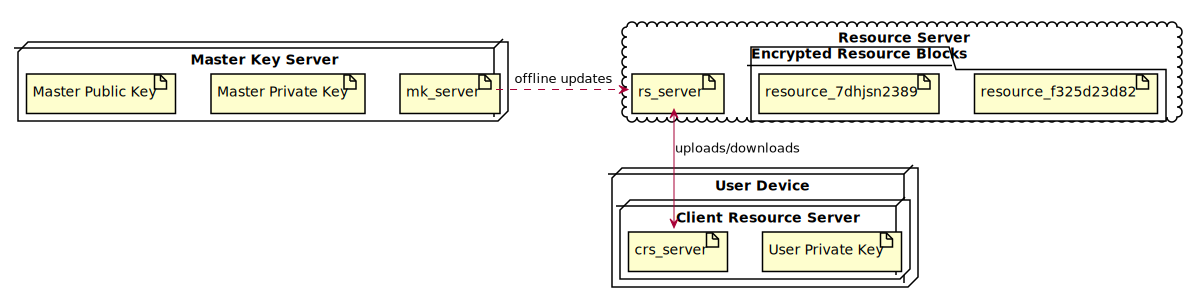
\includegraphics[width=\linewidth,keepaspectratio]{images/infrastructure/deployment_abbrv2.pdf}

  \caption{A second, high-level diagram of the \acrshort{dcs} \theResServer system.}

  \label{fig:deployment_abbrv2_diagram}
\end{figure}

We present the analysis of the deployment scenario and the identified requirements of the \theResServer system along with the enrolment process for new users. From analysis of the \acrfull{dcs} we also present a set of Case Studies, considered by the project throughout design, implementation \& evaluation.

\section{Security Considerations}
\label{sec:analysis_security}

A Resource Server must be built with security as a top priority, or risk resources being vulnerable to attacks and security breaches. Access to resources \textit{can} be managed with Access Control alone, ensuring that only authorised users may view or download a particular resource. Whilst this can meet the basic security needs for a business, no fallback protection is provided in the event of a security breach. Further, within organisations, the security requirements are even higher with more restrictive access and mandatory at-rest encryption being commonplace.

\subsection{Securing Resources}
\label{subsec:analysis_sec_res}

Although open and public resource repositories do exist, such as the \href{https://commons.wikimedia.org/wiki/Main_Page}{Wikimedia Commons} service, they are the edge case across the Internet. A more common setup is a public service with both public and private resources, such as GitHub where code repositories may be set to `private' if a user wishes their code to be hidden from the general public.\\
Files marked as `private' by a user, must remain private and hidden from the general public because a user has a certain expectation that files they upload to a service as `private', cannot be discovered \textbf{or} accessed by other users \textemdash\ unless explicit access has been granted. This expectation must be met by the service or the user's trust is at risk and with it, any future use of the service.
\vskip 0.5em
Access Control is often implemented as the sole method of protecting a user's resources from unauthorised access. This is enough protection for many services, as a user must authenticate to gain access to different routes and locations of a website, with their account dictating if access should be granted or denied. The implications and intricacies of such an authentication system are not within the scope of this project, however the following may provide further information \textemdash\ \citet{Sandhu1996, Johnston2004, Fu2001}.\\
Employment of Access Control as the main defence against unauthorised access works perfectly, until we consider the possibility of a system breach occurring. In such a scenario, the attacker may have broken or circumvented the authentication or authorisation system(s) and gained access to the system's storage. In such a situation, the unencrypted resources are completely vulnerable to the breaching attacker and any restrictions defined by the Access Control system are rendered worthless.\\
\vskip 0.5em
Due to these risks, a system must offer a last line of defence for such situations; a method of protecting the stored resources even when a breach has occurred. In the case of password storage, \citet{Teat2011} show that the risk of breaches is mitigated with cryptographic hashing, however since hashing is a one-way operation we cannot use it for resource storage.\\
Instead we must integrate a form of at-rest encryption to securely store resources as unintelligible binary blobs that cannot be interpreted by man or machine. Such encryption relies on the employment of a block cipher algorithm and the current NIST guidance offers two approved block cipher algorithms \citep{NIST2017}; \acrfull{aes} and Triple DES as described by \citet{Daemen2003} \& \citet{Barker2017}.\\
Unfortunately, both block cipher algorithms are forms of \textit{symmetric}-key encryption which require the same key for encryption and decryption. This usually requires the service provider to store the key(s) separately from the resources and ultimately leaves a single party in control of both keys and encrypted resources, as with Google Drive \& OneDrive business accounts \citep{Winder2018}.

\subsection{Choosing ABE}
\label{subsec:analysis_abe}

\acrfull{abe} by comparison offers the possibility of storing encrypted resources with block cipher algorithms such as \acrshort{aes} 128-bit, yet without the requirement of storing keys. A \textit{ciphertext policy} \acrshort{abe} system for example binds an \acrshort{aes} ciphertext with a policy that describes who shall be able to decrypt it \citep{Akinyele2011} and employs Public Key cryptography (as described in \cref{sec:bkgr_pub_key_infr}) to enforce the policy.\\
In this context, decryption keys are private user keys that have been generated and then signed by a Master Key Server. These keys are generated from a user's attributes, as defined by the organisation, such as (role$=$Staff $\alt$ accountStatus$=$Active $\alt$ department$=$\acrshort{dcs} $\alt$ jobField$=$Research \& Teaching) representing a current member of staff in the Department of Computing Science's Research \& Teaching field.
\vskip 0.5em
Additionally, as an \acrshort{abe} system relies on Public Key cryptography, anyone may encrypt a resource with a policy using the distributed master public key, however only private user keys are capable of decrypting resources. These keys must be generated and then signed by a designated \acrfull{mks} (or private key generator) that remains the only entity with access to the master \textit{private} key. When a user key is created they can be created with a random seed, ensuring that two users with different levels of access cannot collude to form a new key with more access than they have individually \citep{Akinyele2011}, providing implicit \textit{collusion resistance}.\\
Further, Access Control for a service is online only, meaning that if the service is taken offline there is no way for users to access theirs (or other's) resources. By comparison an \acrshort{abe} system requires that access can only be gained through decryption and that files must be decrypted locally \citep{Waters2011}. This means that in the event of the system being inaccessible, users can safely distribute encrypted resources by other means \textemdash\ such as physical transfers \textemdash\ without risking an information breach.

\subsection{ABE Implementation}
\label{subsec:analysis_abe_impl}

To work securely \& efficiently, an \acrshort{abe} system must implement Public Key cryptography as a layer \textit{on top of} a block cipher algorithm such as \acrshort{aes}. Although Public Key cryptography \textemdash\ for example the RSA algorithm \citep{Barker2016} \textemdash\ can encrypt whole resources without \acrshort{aes}, the process is much less efficient and consumes a greater quantity of compute resources in the process \citep{AlHasib2008}. As such, an \acrshort{abe} system should first use \acrshort{aes} to encrypt a resource's contents, producing an \acrshort{aes} \textit{symmetric} key and an encrypted binary blob of the resource.
\vskip 0.5em
Once the key and binary blob have been generated, an \acrshort{abe} system should then use Public Key cryptography to encrypt the key with a Boolean formula policy. An example policy, for the Department of Computing Science and a resource that can only be decrypted by staff members in the Research \& Teaching field, might look like (role(\textbf{s}) $\equiv$ Staff $\wedge{}$ jobField(\textbf{s}) $\equiv$ Research \& Teaching), where \textbf{s} represents the Subject or user attempting to decrypt the related resource.\\
The generated policy should then be embedded directly into the resulting encrypted resource and mathematically bound to the \acrshort{aes} ciphertext with Public Key cryptography, such that it is an absolute requirement that the formula resolve correctly for a provided decryption key \citep{Sahai2005}.
\vskip 0.5em
For the decryption process, the user's attributes are to be extracted from their key and imported into the resource's policy by an \acrshort{abe} system. The system would then attempt to resolve the policy and if and only if the policy resolves to true, the \acrshort{aes} key will be decrypted by the user key. Once the \acrshort{aes} key has been decrypted, the system proceeds to execute \acrshort{aes} decryption on the encrypted binary blob \citep{Akinyele2011}, finally returning an unencrypted resource that can be interpreted by man and machine.


\section{Deployment Considerations}
\label{sec:analysis_deployment}

A service can be designed from the ground up with security in mind, implementing the strongest encryption \& access control mechanisms possible, but if deployed incorrectly the functioning security of the service can be completely undermined.
\vskip 0.5em
The University of Glasgow already provides Microsoft's SharePoint \citep{UofG2019} \& OneDrive \citep{UofG2019a} services as resource-sharing solutions to staff and students, however neither service offers truly granular access control \citep{Microsoft2019} and nor does either service offer a per-department service that the \acrshort{dcs} can implement for only its users.

This lack of granular access means that a user can not share a resource to all users enrolled in the same course, without manually inviting each user individually. By comparison, the \theResServer system would simply require creating a policy that grants access to users that have the attribute associated to that course, such as \texttt{`enrolled\_course \= 2003'}.

\subsection{Security of Public Resource Server}
\label{subsec:analysis_deployment_prs}

The \acrfull{prs} would need to be accessible to all 500+ users in the \acrshort{dcs} (\Cref{appendix:roles_users}) and able to process the uploading \& downloading of all encrypted resources. By design, the resource server would not be aware of the contents of any resources uploaded and would also be unable to execute any encryption or decryption tasks itself. The system would also reject uploads of any resources that are not yet encrypted.

Deployment of the \acrshort{prs} must be publicly accessible to all users in the \acrshort{dcs} and requires a limited level of security. The server does not necessarily require access to the \acrfull{mks} (see \Cref{subsec:analysis_deployment_mks} and \Cref{fig:deployment_diagram}) and can instead rely on manual updates completed via physical transfer by \acrshort{dcs} Admin staff.
\vskip 0.5em
Depending on the desired use, the resource server may be deployed for internal-use only and kept within the \acrshort{dcs} network or deployed with external access via the university's Campus network. Either scenario is considered safe as the resources on the server are implicitly secure due to the at-rest \acrshort{abe}.

Once deployed the system should integreate the university's Single Sign-On authentication system for basic access, which would help defend against attacks and other malicious attempts to disable or damage the system. Further consideration would need to be given to determining a suitable and effective method of completing backups of the encrypted resources but addressing that issue is outwith the scope of the project.

\subsection{Security of Master Key Server}
\label{subsec:analysis_deployment_mks}

Comparatively, the \acrfull{mks} represents the greatest risk to the \theResServer system, as the master \textbf{private} key stored within is capable of generating \& signing any private key. If the \acrshort{mks} becomes compromised, so does the entire system, since the master private key can be maliciously used to generate any arbitrary decryption key.

To combat this risk, the \acrshort{mks} is designed to be kept `offline' after initial setup is complete and the whole system has been successfully provisioned. This drastically reduces attack vectors to the server.

\begin{figure}[htp]
    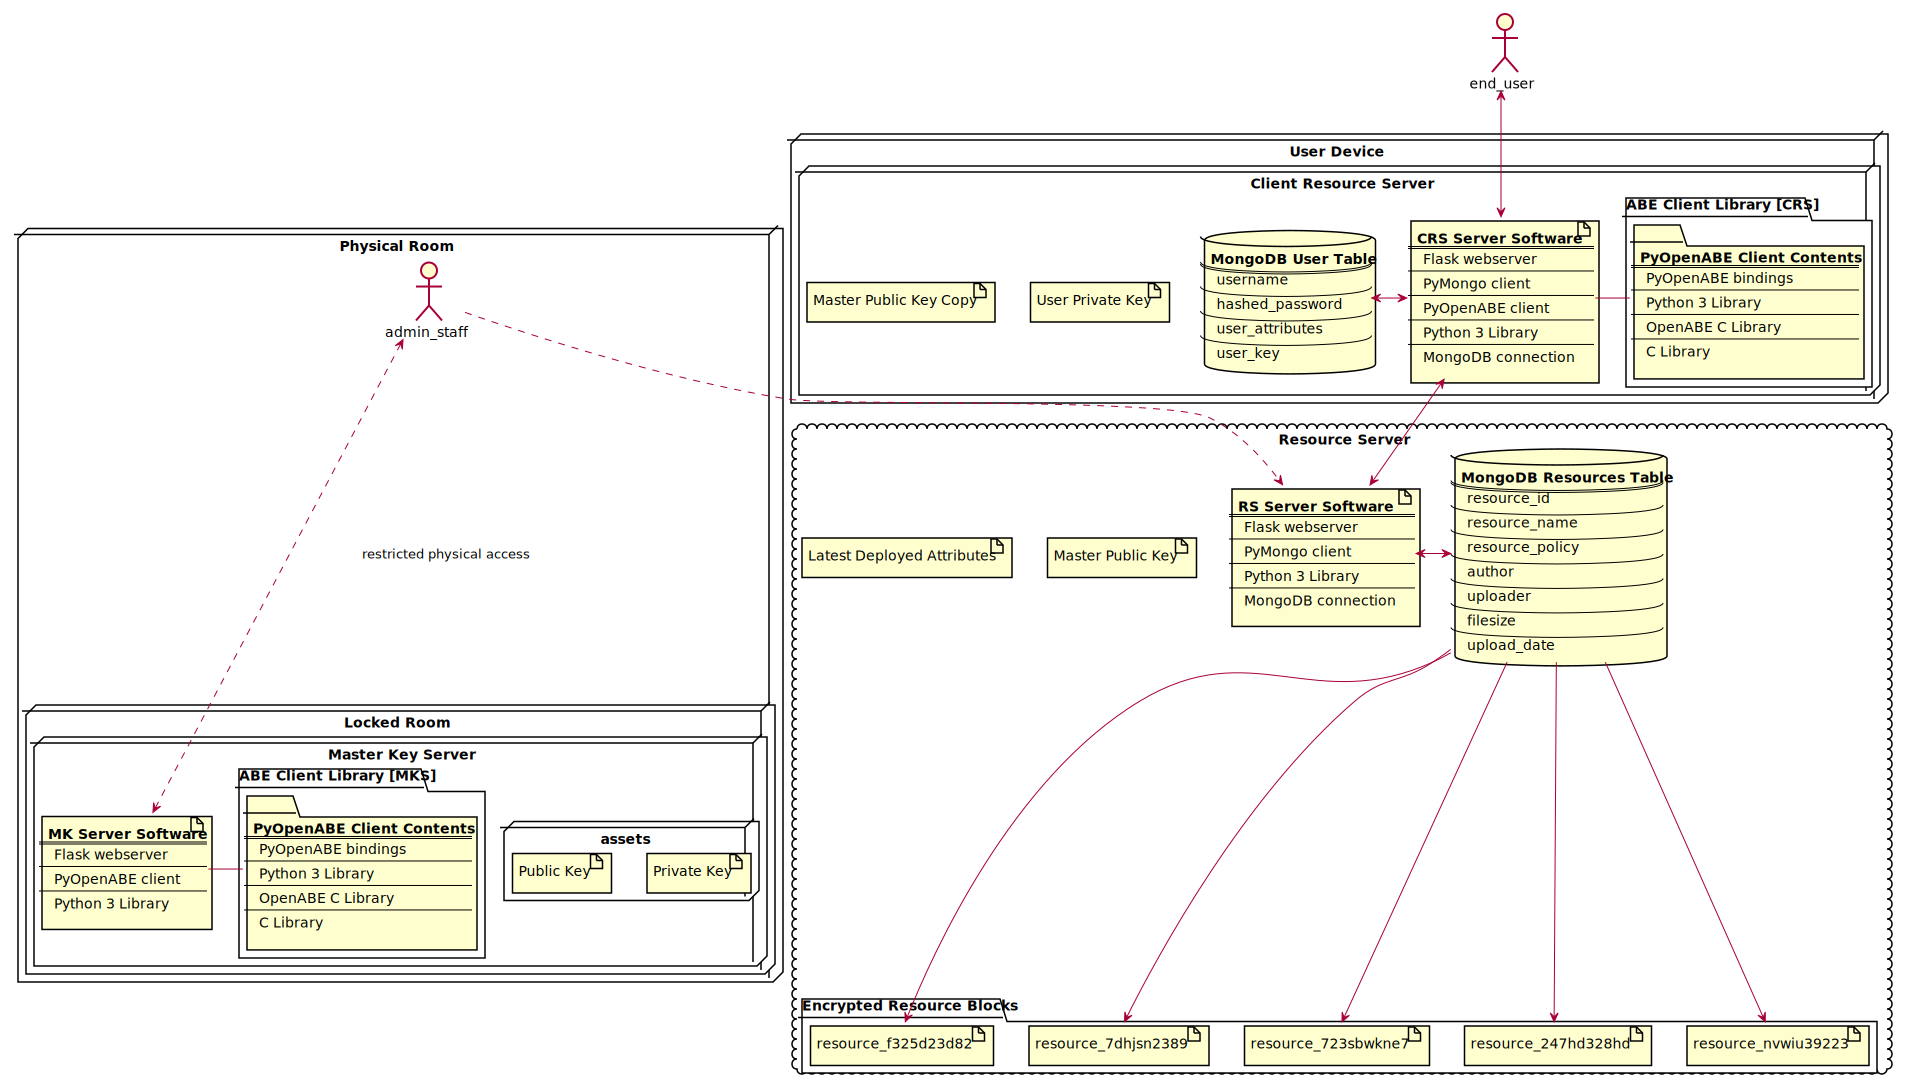
\includegraphics[width=\linewidth,keepaspectratio]{images/infrastructure/deployment.pdf}

    \caption{A deployment diagram of the \acrshort{dcs} \theResServer system. Both servers can be seen in context, with the \acrfull{mks} in its `offline' state and with physical access restricted to Admin staff. The \acrlong{prs} is shown receiving physical updates from the \acrshort{mks} (handled by Admin Staff) and communicating with a \acrlong{crs} running on a user's local device.}

    \label{fig:deployment_diagram}
\end{figure}

Physical access to the \acrshort{mks} remains a high risk concern. It was thus determined that physical access to the server must also be restricted, meaning the \acrshort{mks} would be deployed in a physically locked room with access only granted to \acrshort{dcs} Admin staff, as shown in \Cref{fig:deployment_diagram}.

The \acrshort{mks} would run on a UNIX \acrshort{os}, allowing for user authentication and system logging of events. Thus, in the event of a physical breach of security, a rogue party could not access the \acrshort{mks} to issue new keys. Additionally, if a rogue member of staff generates false keys, they would leave an auditable trail.

\subsection{Issuing User Keys}
\label{subsec:analysis_deployment_iuk}

From \Cref{subsec:analysis_deployment_mks}, the \acrfull{mks} generates \& signs decryption keys for the \theResServer system, using the stored master \textbf{private} key. Further, as discussed in \Cref{subsec:analysis_abe}, the decryption keys for the system are private user keys which contain embedded attributes that describe a user.

\begin{figure}[htp]
    \centering
    \includegraphics[width=\linewidth,keepaspectratio]{images/flow_of_info/enrollment_stu_sequence.pdf}

    \caption{A sequence diagram demonstrating the \theResServer enrolment process for a student.}

    \label{fig:enrolment_diagram}
\end{figure}

A user may enrol into the \theResServer system, by having a member of the \acrshort{dcs} Admin staff generate \& sign a new user key with their personal details from the \acrshort{mks}, see  and Appendix \ref{appendix:enrolment_diagram}.

\Cref{fig:enrolment_diagram} shows a student requesting a user key from the \acrshort{dcs} Teaching Assistant, whom verifies the student's identity and then retrieves their details from the Student Centre. The Teaching Assistant then processes the returned attributes for the \acrshort{mks}, and then requests a new key by providing the student's attributes. The \acrshort{mks} can be seen processing and then returning the newly generated key to the Teaching Assistant, whom finally provides the key to the student.
\vskip 0.5em
The \acrshort{mks} would be designed to \textit{validate} the attributes of a new user to ensure compatibility with encrypted resources and that all generated user keys are comparable. The \acrshort{mks} would not be designed to \textit{verify} the attributes of a new user.

It is instead assumed that the Admin staff are responsible for verifying both the identity of a user and that the attributes about to be assigned to them are correct; meaning both physical and login access to the \acrshort{mks} \textit{must only} be granted to trained members of staff.

The Admin staff member must physically transfer the newly created key from the \acrshort{mks} to the user via some form of hardware storage, such as a USB flash drive. Care would have to be taken to ensure that the \acrshort{mks} cannot become infected from malicious storage devices.


\section{Enrolment Requirements}
\label{sec:analysis_enrolment}

Following from \cref{subsec:analysis_deployment_mks} and \cref{subsec:analysis_deployment_iuk}, a Department of Computing Science user must be able to enrol in the \theResServer system by physically visiting the Teaching Office and proving their identity to the Admin staff. Staff and students could prove their identity with their respective campus ID cards, with passports providing further evidence should the Admin staff require it.\\
Any member of the \acrfull{dcs} would be eligible for enrolment in the system as long as they were able to adequately prove their membership to the Admin staff. This process would be deliberately designed to be partly physical for the added security in transferring the user's new key via a physical storage medium (instead of an electronic system such as email) as well as aiding the identity verification process with the user's physical presence.\\
New members of the \acrshort{dcs} must already physically attend an appointment to activate their campus cards for access to \acrshort{dcs} buildings \& laboratories, meaning that the \theResServer enrolment could reasonably be added to this process for limited impact on new users. Current users would have to visit the Teaching Office to complete enrolment into the system, however appointments could be timetabled and managed to ensure the smallest possible impact on \acrshort{dcs} members.


\section{Case Studies}
\label{sec:analysis_case_studies}

From the work completed in \cref{ch:background} and sections \ref{sec:analysis_security}, \ref{sec:analysis_deployment} \& \ref{sec:analysis_enrolment}, the project had determined the users of the resource server as well as the features the service would need to provide. With this information, several Case Studies were designed to demonstrate the extensibility of the system in real-world scenarios. Of the 6 Case Studies presented here, \cref{subsec:analysis_case_studies_3} and \cref{subsec:analysis_case_studies_5} are examined and discussed at the most in-depth level.

\subsection{\#1 - Course Lecture Slides}
\label{subsec:analysis_case_studies_1}

Case Study \#1 considers a set of Lecture Slides uploaded as an encrypted resource by the Lecturer of an arbitrary course. For the sake of the scenario however, the Java Programming 2 course was selected with Course Code 2001 in order to demonstrate the creation of a policy.
\vskip 0.5em
For this study it should be noted that:
\begin{itemize}
  \item
    the lecture slides have been uploaded in advance of the lecture date
  \item
    the lecture date is scheduled for 23/10/19
  \item
    the solutions were encrypted and then uploaded by the Lecturer
  \item
    the Lecturer for 2001 is Jeremy Springer with username `jspringer'
  \item
    Course 2001 is a Level 2 course
\end{itemize}
\vskip 0.5em
From the above information, the following attributes can be extracted for the policy, where we define \textbf{\textit{Subject} s} and \textbf{\textit{Environment} e} as:
\begin{itemize}
  \item[]
    \textbf{s} $\Rightarrow$ role, jobField, studentLevel, enrolledCourses, accountActiveUntil, username
  \item[]
    \textbf{e} $\Rightarrow$ currentDate
\end{itemize}

Applying the above attributes for the scenario provides the policy in \cref{fig:case_study_policy_1} which would have been embedded in the encrypted lecture slides by the Lecturer prior to upload. The encrypted slides can then remain stored on the server but only accessible to Research \& Teaching staff members until 24 hours before the lecture date of 23/10/19, when students on the course will also be granted access.

\begin{figure}[ht]
  \centering
\begin{align*}
  \text{Policy(\textbf{s},\textbf{e})}
  &
    \leftarrow
    \text{username(\textbf{s})} \equiv \text{jspringer}
  \\
  &
    \vee
    \text{( role(\textbf{s})} \equiv \text{Staff}
  \\
  &
    \phantom{::}\phantom{::}\wedge
    \text{jobField(\textbf{s})} \equiv \text{Research \& Teaching )}
  \\
  &
    \vee
    \text{( role(\textbf{s})} \equiv \text{Student}
  \\
  &
    \phantom{::}\phantom{::}\wedge
    \text{studentLevel(\textbf{s})} \equiv \text{2}
  \\
  &
    \phantom{::}\phantom{::}\wedge
    \text{enrolledCourses(\textbf{s})} \equiv \text{2001}
  \\
  &
    \phantom{::}\phantom{::}\wedge
    \text{currentDate(\textbf{e})} \geq \text{22 October 2019 )}
  \\
  &
    \wedge
    \text{accountActiveUntil(\textbf{s})} \geq \text{currentDate(\textbf{e})}
\end{align*}
  \caption{
    \label{fig:case_study_policy_1}
    Case Study \#1 policy dictating access to a set of course 2001 lecture slides.
    Successful decryption would be possible for the author of the slides (with username `jspringer') \textbf{or} a member of staff in the Research \& Teaching field \textbf{or} a Level 2 student enrolled in the 2001 course if the lecture slides' release date has passed. In all cases an active account is also required.
  }
\end{figure}

\subsection{\#2 - Course Lab Solutions}
\label{subsec:analysis_case_studies_2}

Case Study \#2 considers a lab solution uploaded as an encrypted resource by the Lecturer of an arbitrary course. For the sake of the scenario however, the 1P Programming course was selected with Course Code 1001 as it has the added complexity of tutors \& demonstrators, but it should be remembered that any course with labs could have been chosen.
\vskip 0.5em
For this study it should be noted that:
\begin{itemize}
  \item
    the lab solutions have been uploaded in advance of the actual lab date
  \item
    the lab date is scheduled for 04/12/19
  \item
    the solutions were encrypted and then uploaded by the Lecturer
  \item
    the Lecturer for 1001 is John Williamson with username `jwilliamson'
  \item
    Course 1001 is a Level 1 course
  \item
    Course 1001 has a sister course, 1017
  \item
    the 1P course labs are assisted by tutors \& demonstrators from Level 4+
\end{itemize}
\vskip 0.5em
From the above information, the following attributes can be extracted for the policy, where we define \textbf{\textit{Subject} s} and \textbf{\textit{Environment} e} as:
\begin{itemize}
  \item[]
    \textbf{s} $\Rightarrow$ role, jobField, studentLevel, enrolledCourses, accountActiveUntil, startDate, endDate, username, studentRole, demonstratorCourses
  \item[]
    \textbf{e} $\Rightarrow$ currentDate
\end{itemize}

Applying the above attributes for the scenario provides the policy in \cref{fig:case_study_policy_2} which would have been embedded in the encrypted lab solution by the Lecturer prior to upload. The encrypted lab solution can then remain stored on the server but only accessible to Research \& Teaching staff members and valid tutors \& demonstrators until 3 days after the lab date of 04/12/19, when students on the course will also be granted access.

\begin{figure}[ht]
  \centering
\begin{align*}
  \text{Policy(\textbf{s},\textbf{e})}
  &
    \leftarrow
    \text{username(\textbf{s})} \equiv \text{jwilliamson}
  \\
  &
    \vee
    \text{( role(\textbf{s})} \equiv \text{Staff}
  \\
  &
    \phantom{::}\phantom{::}\wedge
    \text{jobField(\textbf{s})} \equiv \text{Research \& Teaching )}
  \\
  &
    \vee
    \text{( role(\textbf{s})} \equiv \text{Student}
  \\
  &
    \phantom{::}\phantom{::}\wedge
    \text{studentLevel(\textbf{s})} \equiv \text{1}
  \\
  &
    \phantom{::}\phantom{::}\wedge
    \text{enrolledCourses(\textbf{s})} \equiv \text{1001, 1017}
  \\
  &
    \phantom{::}\phantom{::}\wedge
    \text{currentDate(\textbf{e})} \geq \text{7 December 2019 )}
  \\
  &
    \vee
    \text{( role(\textbf{s})} \equiv \text{Student}
  \\
  &
    \phantom{::}\phantom{::}\wedge
    \text{studentLevel(\textbf{s})} \equiv \text{4} \mid \text{M} \mid \text{PG}
  \\
  &
    \phantom{::}\phantom{::}\wedge
    \text{studentRole(\textbf{s})} \equiv \text{Demonstrator UG} \mid \text{Demonstrator PG} \mid \text{Tutor}
  \\
  &
    \phantom{::}\phantom{::}\wedge
    \text{demonstratorCourses(\textbf{s})} \equiv \text{1001, 1017}
  \\
  &
    \phantom{::}\phantom{::}\wedge
    \text{startDate(\textbf{e})} \leq \text{currentDate(\textbf{e})}
  \\
  &
    \phantom{::}\phantom{::}\wedge
    \text{endDate(\textbf{e})} \geq \text{currentDate(\textbf{e}) )}
  \\
  &
    \wedge
    \text{accountActiveUntil(\textbf{s})} \geq \text{currentDate(\textbf{e})}
\end{align*}
  \caption{
    \label{fig:case_study_policy_2}
    Case Study \#2 policy dictating access to a set of course 1001 lab solutions.
    Successful decryption would be possible for the author of the solutions (with username `jwilliamson') \textbf{or} a member of staff in the Research \& Teaching field \textbf{or} a Level 2 student enrolled in the 1001 \& 1017 courses if the lab date has passed \textbf{or} a Level 4+ student employed as a demonstrator or tutor that has been assigned to 1001 \& 1017 and it is within their dates of employment. In all cases an active account is also required.
  }
\end{figure}

\subsection{\#3 - In-progress Exam Script}
\label{subsec:analysis_case_studies_3}

\subsection{\#4 - Past Paper}
\label{subsec:analysis_case_studies_4}

\subsection{\#5 - Level 4 Student Project}
\label{subsec:analysis_case_studies_5}

\subsection{\#6 - Class Rep Meeting Minutes}
\label{subsec:analysis_case_studies_6}


\section{Summary}
\label{sec:analysis_summary}

With analysis of the \acrfull{dcs} deployment presented, we presented the security considerations of the \theResServer system, discussing the requirement of securing uploaded resources and the reasons the project selected \acrfull{abe} for this purpose, including the integration with \acrshort{abe}.

We also presented the individual security considerations of both the \acrfull{prs} and \acrfull{mks} in the context of the \acrshort{dcs}, along with the enrolment process for new users (accounting for the offline status of the \acrshort{mks}).

Finally, we described the six Case Studies for the \theResServer system and demonstrated the applicability of each study to the \acrshort{dcs}.

%==================================================================================================================================
\chapter{Design}
\label{ch:design}

With Background (\Cref{ch:background}) and Analysis (\Cref{ch:analysis}) presented, we present the design of the \theResServer system and the design requirements for the different aspects of the system.\\
This includes the formal language definition (\Cref{sec:formal_lang}) for \theResServer system's policy language, \thePolicyLang, the design of the system's User Keys (\Cref{sec:design_user_key}) and the System Architecture (\Cref{sec:design_sys_arch}). Further, we present the design of the Policy Building (\Cref{sec:design_pol_build}) \& Filename Searching (\Cref{sec:design_file_search}) tools to be incorporated into the \acrfull{crs}.

\section{Requirements}
\label{sec:design_reqs}

\subsection{Deployment}
\label{subsec:design_deployment}

The \theResServer system is designed around the specific deployment scenario of the \acrfull{dcs} and as such, aims to meet the requirements of users belonging to the \acrshort{dcs}. Identified by an analysis of the \acrshort{dcs} structure, considering students, teaching staff, technical \& admin staff and identifying both key roles and individuals within the organisation (see \cref{appendix:roles_users}).\\
Meaning that the \theResServer system focuses on the secure distribution of resources between members of a department with particular emphasis on the sharing of course resources between members of staff and the students taking their course(s).
\vskip 0.5em
This scenario also lends itself well to proving the extensibility of the product as students have varying and changing attributes that are assigned in their private user keys \textemdash\ the dynamic nature of which allows the product to maintain a high level of portability.\\
This granularity in attributes, and thus policies, also provides long-term support for the product by allowing it to adapt to future changes in user structure and policy requirements. Furthermore, the system is can also be deployed in completely new environments as the attributes can be unique to an industry and do not require complete definition before deployment.
\vskip 0.5em
The product was thus determined to require one central \acrfull{mks}, tasked with maintaining the master private key, provisioning the corresponding master public key and using said private key to sign new user keys.\\
A second server would handle the distribution of the master public key, storage of the encrypted resources and serving \& receiving encrypted resources.\\
Further, it was determined that for the \acrshort{dcs} deployment, the \acrshort{mks} would serve as an offline or 'cold' server with no network connection; as this provides a strong level of base security against external threats. Such offline status is possible because the \acrshort{mks} is not required to distribute data automatically, but rather the master public key can be manually uploaded to the \acrfull{prs}.

\subsection{\acrshort{abe} System}
\label{subsec:design_abe_sys}

An \acrfull{abe} system requires a defined policy language for building the policies that resources will be encrypted with. This policy language, \thePolicyLang, is defined in \cref{sec:formal_lang} and describes the syntax \& types for policies. It is tailored to the deployment described above by allowing for attributes that are required for students and staff of the \acrshort{dcs}.\\
The \acrshort{abe} system required an \acrshort{abe} library for employment and since creating such a library was beyond the scope of the project, the \href{https://github.com/zeutro/openabe}{\OpenABE library} from Zeutro LLC was selected instead (see \cref{sec:bkgr_openabe} for more information). \OpenABE was selected based upon the open source philosophy it adopts and the demonstration of its deployment as an electronic medical record system \citet{Akinyele2011} \textemdash\ a system that aligns well with that of a secure, departmental resource server but with even greater requirements for security.

\subsection{Resources}
\label{subsec:design_resources}

Since uploaded resources have to be securely encrypted with \acrshort{abe} before transmission, the \acrfull{prs} is unaware of the contents of all resources and is in the disadvantaged position of being unable to help users identify which resources are which.\\
As such, the server must utilise a different method for resource identification, instead relying on an internal database to store metadata of resources as provided when a user performs an upload. This metadata includes filename, extension, file size and author, but most importantly keeps a record of the resource's policy, allowing the system to determine if a user should even be able to download the resource. Additionally, the metadata stored is entirely extensible and could be further extended in future as needs evolve.\\
Importantly, any user \textit{could} download \textit{any} encrypted resource without risk of unauthorised decryption, however the user experience would be degraded due to an overwhelming visibility of all uploaded resources. As such, a simple Access Control (see \cref{sec:bkgr_acc_ctrl}) system was built into the system to only offer visibility to resources a user may download \& decrypt successfully.


\section{Formal Language Definition}
\label{sec:formal_lang}
The formal language definition for the Attribute-Based Encryption policy language, \thePolicyLang.

\subsection{Abstract Syntax, Types, \& Contexts}
\label{subsec:defs}

\begin{figure}[ht]
  \centering
\begin{align*}
  \ty{n}{\mathbb{Z}}
  &
    \Coloneqq
    \text{Integers}
  & \text{Values}
  \\
  \ty{b}{\mathbb{B}}
  & \Coloneqq
    \mathsf{False}\alt\mathsf{True}
  \\
  \ty{d}{\mathbb{D}}
  & \Coloneqq
    \text{Dates}
  \\
  \ty{s}{\mathbb{S}}
  & \Coloneqq
    \text{Strings}
  \\
  v
  &
    \Coloneqq
    n
    \alt
    b
    \alt
    d
    \alt
    s
  \\
  \ty{l}{\mathbb{L}_T}
  & \Coloneqq
    \emptyset_T\alt{}v\Cons_T{}l
  \\
  e
  &
    \Coloneqq
    v
    \alt
    l
  & \text{Expressions}
  \\
  &
    \firstAlt
    \exprEQ{e}{e}
    \alt
    \exprGT{e}{e}
    \alt
    \exprLT{e}{e}
  \\
  & \firstAlt
    \exprGTE{e}{e}
    \alt
    \exprLTE{e}{e}
  &
  \\
  & \firstAlt
    \exprOr{e}{e}
    \alt
    \exprAnd{e}{e}
  &
  \\
  &
    \firstAlt
    \left( \lambda \mu \bullet e \right)
    \alt
    e \; \$ \; e
  &
    \text{Statements}
  \\
  T
  &
    \Coloneqq
    \mathbb{Z}
    \alt
    \mathbb{B}
    \alt
    \mathbb{D}
    \alt
    \mathbb{S}
    \alt
    \mathbb{L}
  &
    \text{Types}
  \\
  \Gamma
  &
    \Coloneqq
    \envAdd{(\ty{x}{T})}
    \alt
    \emptyset
    &
      \text{Context}
\end{align*}
  \caption{\label{fig:syntax}\thePolicyLang abstract syntax, types, and context.}
\end{figure}

\Cref{fig:syntax} presents the syntactical structure, and types for our language.
Our language contains Integers, Boolean, Date, String and List values, we leave abstract how integers and dates are written. Lists may either be empty or consist of any number of elements where each element is of the same type $T \in v$.

Integers \& Dates can be compared using standard comparison operations of: \texttt{greater-than}, \texttt{less-than} and \texttt{equals-to}, as well as \texttt{greater-than-or-equal-to} and \texttt{less-than-or-equal-to}.
Boolean operators provide logical conjunction and disjunction.

A context ($\Gamma$) keeps track of well-typed expressions, and our context can be expanded.


\subsection{Typing Rules}
\label{subsec:typing-rules}

\begin{figure}[ht]
  \centering
\begin{mathpar}
  \infer*[left=Intro-Int]
  {
    \\
  }
  {
    \ty{i}{\TyInt}
  }
  \and
  \infer*[left=Intro-Bool]
  {
    \\
  }
  {
    \ty{b}{\mathbb{B}}
  }
  \and
  \infer*[left=Intro-Date]
  {
    \\
  }
  {
    \ty{d}{\mathbb{D}}
  }
  \and
  \infer*[left=Intro-String]
  {
    \\
  }
  {
    \ty{s}{\mathbb{S}}
  }
  \and
  \infer*[left=Intro-List]
  {
    \\
  }
  {
    \ty{l}{\mathbb{L}_T}
  }
  \and
  \infer*[left=OR]
  {
    \env{\ty{a}{\mathbb{B}}}\\
    \env{\ty{b}{\mathbb{B}}}
  }
  {
    \env{\ty{\exprOr{a}{b}}{\mathbb{B}}}
  }
  \and
  \infer*[left=AND]
  {
    \env{\ty{a}{\mathbb{B}}}\\
    \env{\ty{b}{\mathbb{B}}}
  }
  {
    \env{\ty{\exprAnd{a}{b}}{\mathbb{B}}}
  }
  \and
  \infer*[left=GT]
  {
    \env{\ty{a}{T}}\\
    \env{\ty{b}{T}}\\
    \left[ T \in \{ \mathbb{Z}, \mathbb{D} \} \right]
  }
  {
    \env{\ty{\exprGT{a}{b}}{\mathbb{B}}}
  }
  \and
  \infer*[left=LT]
  {
    \env{\ty{a}{T}}\\
    \env{\ty{b}{T}}\\
    \left[ T \in \{ \mathbb{Z}, \mathbb{D} \} \right]
  }
  {
    \env{\ty{\exprLT{a}{b}}{\mathbb{B}}}
  }
  \and
  \infer*[left=EQ]
  {
    \env{\ty{a}{T}}\\
    \env{\ty{b}{T}}\\
    \left[ T \in \{ \mathbb{Z}, \mathbb{B}, \mathbb{D}, \mathbb{S}, \mathbb{L}_T \} \right]
  }
  {
    \env{\ty{\exprEQ{a}{b}}{\mathbb{B}}}
  }
  \and
  \infer*[left=GTE]
  {
    \env{\ty{a}{T}}\\
    \env{\ty{b}{T}}\\
    \left[ T \in \{ \mathbb{Z}, \mathbb{D} \} \right]
  }
  {
    \env{\ty{\exprGTE{a}{b}}{\mathbb{B}}}
  }
  \and
  \infer*[left=LTE]
  {
    \env{\ty{a}{T}}\\
    \env{\ty{b}{T}}\\
    \left[ T \in \{ \mathbb{Z}, \mathbb{D} \} \right]
  }
  {
    \env{\ty{\exprLTE{a}{b}}{\mathbb{B}}}
  }
\end{mathpar}
  \caption{\label{fig:rules}The formal definiton of the Typing Rules for \thePolicyLang}
\end{figure}

\Cref{fig:rules} presents the \thePolicyLang typing rules.
These rules dictate what it means for an expression/statement to be well-formed within \thePolicyLang and for any expression/statement in \thePolicyLang, we use the typing rules to construct a derivation that provides proof that the expression/statement is well-typed, that is we can apply each rule and form a derivation tree. If we cannot construct this tree then the expression is ill-typed and syntactically not valid.\\
The Typing Rules define 5 base cases for the 5 value types \thePolicyLang supports (as defined in \cref{fig:syntax}), meaning instances of the 5 types derive directly to their type. Next, the boolean logical operators OR \& AND are defined as requiring two Boolean parameters that also derive to a Boolean type return. The standard comparison operators \textbf{greaterThan}, \textbf{lessThan}, \textbf{greaterThanEqual} \& \textbf{lessThanEqual} all take two parameters of a matching type, where the type may be Integer or Date, and derives to a Boolean response. Lastly, the \textbf{equal} comparison similarly takes two paramters of a matching type, but where the type may be Integer, Boolean, Date, String or List, and also derives to a Boolean return.


\subsection{Substitution}
\label{subsec:substitution}

\begin{figure}[ht]
  \centering
\begin{align*}
  \subst{\mu}{e}{x}
  &
    \Coloneqq
    \begin{cases}
      e&x\equiv\mu\\
      x&x\not\equiv\mu\\
    \end{cases}
  \\
  \subst{\exprOr{a}{b}}{e}{x}&\Coloneqq\exprOr{\subst{a}{e}{x}}{\subst{b}{e}{x}}\\
  \subst{\exprAnd{a}{b}}{e}{x}&\Coloneqq\exprAnd{\subst{a}{e}{x}}{\subst{b}{e}{x}}\\
  \subst{\exprGT{a}{b}}{e}{x}&\Coloneqq\exprGT{\subst{a}{e}{x}}{\subst{b}{e}{x}}\\
  \subst{\exprLT{a}{b}}{e}{x}&\Coloneqq\exprLT{\subst{a}{e}{x}}{\subst{b}{e}{x}}\\
  \subst{\exprEQ{a}{b}}{e}{x}&\Coloneqq\exprEQ{\subst{a}{e}{x}}{\subst{b}{e}{x}}\\
  \subst{\exprGTE{a}{b}}{e}{x}&\Coloneqq\exprGTE{\subst{a}{e}{x}}{\subst{b}{e}{x}}\\
  \subst{\exprLTE{a}{b}}{e}{x}&\Coloneqq\exprLTE{\subst{a}{e}{x}}{\subst{b}{e}{x}}
\end{align*}
  \caption{\label{fig:subst}The formal definition of the Substitution Rules for \thePolicyLang}
\end{figure}

\Cref{fig:subst} presents a standard set of substitution rules for \thePolicyLang.
These rules describe how we can iterate over our expressions/statements in \thePolicyLang and through recursive calls, swap variables for values.

Starting with expressions and variables, we describe when $\mu$ is an expression or variable. Next we describe the resolving of the \textbf{or} \& \textbf{and} logical operators' parameters to expressions and variables, followed by similar descriptions for the standard comparisons \textbf{greaterThan}, \textbf{lessThan}, \textbf{equal}, \textbf{greaterThanEqual} \& \textbf{lessThanEqual}.


\section{Big Step Semantics}\label{sec:semantics}

\begin{figure}[ht]
  \centering
\begin{mathpar}
  \infer*[left=Nat]
  {
    \\
  }
  {
    n\Downarrow{}n
  }
  \and
  \infer*[left=$\mathbb{B}$]
  {
    \\
  }
  {
    b\Downarrow{}b
  }
  \and
  \infer*[left=$\mathbb{D}$]
  {
    \\
  }
  {
    d\Downarrow{}d
  }
  \and
  \infer*[left=$\mathbb{S}$]
  {
    \\
  }
  {
    s\Downarrow{}s
  }
  \and
  \infer*[left=$\mathbb{L}$]
  {
    \\
  }
  {
    l\Downarrow{}l
  }
  \and
  \infer*[left=OR]
  {
    a\Downarrow{}\primed{a}\\
    b\Downarrow{}\primed{b}
  }
  {
    \exprOr{a}{b}\Downarrow\primed{a}\vee\primed{b}
  }
  \and
  \infer*[left=AND]
  {
    a\Downarrow{}\primed{a}\\
    b\Downarrow{}\primed{b}
  }
  {
    \exprAnd{a}{b}\Downarrow\primed{a}\wedge\primed{b}
  }
  \and
  \infer*[left=GT]
  {
    a\Downarrow{}\primed{a}\\
    b\Downarrow{}\primed{b}
  }
  {
    \exprGT{a}{b}\Downarrow\primed{a}>\primed{b}
  }
  \and
  \infer*[left=LT]
  {
    a\Downarrow{}\primed{a}\\
    b\Downarrow{}\primed{b}
  }
  {
    \exprLT{a}{b}\Downarrow\primed{a}<\primed{b}
  }
  \and
  \infer*[left=EQ]
  {
    a\Downarrow{}\primed{a}\\
    b\Downarrow{}\primed{b}
  }
  {
    \exprEQ{a}{b}\Downarrow\primed{a}\equiv\primed{b}
  }
  \and
  \infer*[left=GTE]
  {
    a\Downarrow{}\primed{a}\\
    b\Downarrow{}\primed{b}
  }
  {
    \exprGTE{a}{b}\Downarrow\primed{a}\geqq\primed{b}
  }
  \and
  \infer*[left=LTE]
  {
    a\Downarrow{}\primed{a}\\
    b\Downarrow{}\primed{b}
  }
  {
    \exprLTE{a}{b}\Downarrow\primed{a}\leqq\primed{b}
  }
  \and
  \infer*[left=Let]
  {
    e_1\Downarrow\primed{e_1}\\
    \subst{e_2}{\mu}{\primed{e_1}}\Downarrow\primed{e_2}
  }
  {
    \stmtLet{\mu}{{e}_{1}}{e_{2}}\Downarrow\primed{e_2}
  }\end{mathpar}
  \caption{\label{fig:semantics}Big Step Semantics}
\end{figure}

Operational semantics describe how we evaluate our programs.
This describes how we can \emph{reduce}/evaluate our language expressions and statements to a single value.
There are generally two common styles of operational semantics: Big-Step, and Small-Step.
There are more formal names given but we generally refer to the styles using these names.

Big-Step semantics are concerned with what the final result is; we can skip description of intermediate computations.
Small-Step semantics are concerned with how we get to the final result; we cannot skip intermediate computations.
Both have pros and cons.

\Cref{fig:semantics} presents Big-Step style semantics, here we use \emph{real} operations to show how an expression is reduced using \emph{real} integer and boolean operators.


\subsection{Interpretation}
\label{subsec:interpretation}

\begin{figure}[ht]
  \centering
\begin{align*}
  \textsc{\thePolicyLang}&\rightarrow\textsc{Python (PyOpenABE)}\\
  \interpB{\TyInt}&\Coloneqq\text{\ttfamily int}\\
  \interpB{\mathbb{B}}&\Coloneqq\text{\ttfamily bool}\\
  \interpB{\mathbb{D}}&\Coloneqq\text{\ttfamily datetime.date}\\
  \interpB{\mathbb{S}}&\Coloneqq\text{\ttfamily str}\\
  \interpB{\mathbb{L}}&\Coloneqq\text{\ttfamily list}\\
  \interpB{n}&\Coloneqq\text{\ttfamily int(}n\text{\ttfamily)}\\
  \interpB{\EnumFalse}&\Coloneqq\text{\ttfamily False}\\
  \interpB{\EnumTrue} &\Coloneqq\text{\ttfamily True}\\
  \interpB{d}&\Coloneqq\text{\ttfamily datetime.date(}d\text{\ttfamily)}\\
  \interpB{s}&\Coloneqq\text{\ttfamily str(}s\text{\ttfamily)}\\
  \interpB{l}&\Coloneqq\text{\ttfamily [}l\text{\ttfamily]}\\
  \interpB{\exprOr{a}{b}}  &\Coloneqq\interpB{a}\,\text{\ttfamily or}\,\interpB{b}\\
  \interpB{\exprAnd{a}{b}} &\Coloneqq\interpB{a}\,\text{\ttfamily and}\,\interpB{b}\\
  \interpB{\exprGT{a}{b}}  &\Coloneqq\interpB{a}\,\text{\ttfamily \textgreater}\,\interpB{b}\\
  \interpB{\exprLT{a}{b}}  &\Coloneqq\interpB{a}\,\text{\ttfamily \textless}\,\interpB{b}\\
  \interpB{\exprEQ{a}{b}}  &\Coloneqq\interpB{a}\,\text{\ttfamily ==}\,\interpB{b}\\
  \interpB{\exprGTE{a}{b}}  &\Coloneqq\interpB{a}\,\text{\ttfamily \textgreater =}\,\interpB{b}\\
  \interpB{\exprLTE{a}{b}}  &\Coloneqq\interpB{a}\,\text{\ttfamily \textless =}\,\interpB{b}
\end{align*}
  \caption{\label{fig:interp}The formal definiton of the Interpretation Rules for \thePolicyLang}
\end{figure}

In this final section we describe how we interpret \thePolicyLang to another form, in this case concrete Python expressions for the PyOpenABE bindings library (described in \cref{subsec:bkgr_pyopenabe}).\\
\Cref{fig:interp} presents these Interpretation rules for \thePolicyLang and like substitution, interpretation recursively operates over each statement and expression in \thePolicyLang. At each step replacing the expression from \thePolicyLang with it's equivalent Python form. As we are interpreting \thePolicyLang we do not provide operational semantics, since Python provides this for us.



\section{Formal Language Definition}
\label{sec:formal_lang}

We offer the following formal language definition for the \theResServer system's \acrfull{abe} policy language, \thePolicyLang. The language is designed around the Case Studies described in \Cref{sec:analysis_case_studies} and follows an extensible design principle that aims to provide a complete policy solution for the \acrfull{dcs}.

\thePolicyLang allows for policies to be constructed for the \Cref{sec:analysis_case_studies} Case Studies, which can then be interpreted to the policy format that the \PyOpenABE python bindings (described in \Cref{sec:bkgr_openabe}) require.
\vskip 0.5em
\thePolicyLang offers Boolean comparisons for Integer, String \& Date attributes with further support for Lists of multiple values. Additional comparison operations are provided for Integer and Date comparisons with `greater than', `less than' and `equivalent to' all supported, whereas Booleans, Strings and Lists support `equivalent to' operations only.

This allows for Integer comparisons such as ``\textit{studentLevel(\textbf{s}) $\geq$ 4}'' (as found in Case Study \#2, \Cref{fig:case_study_policy_2}) and Date comparisons such as ``\textit{classRepFrom(\textbf{s}) $\geq$ 17 Sep 2019}'' (as found in Case Study \#5, \Cref{fig:case_study_policy_5}). String equivalence operations allow for comparisons such as ``\textit{jobField(\textbf{s}) $\equiv$ `Research \& Teaching'}'' (as found in Case Study \#1, \Cref{fig:case_study_policy_1}).

List equivalence operations are also supported, allowing for comparisons such as ``\textit{enrolledCourses(\textbf{s}) $\equiv$ [1001, 1017]}'' (as found in Case Study \#2 \Cref{fig:case_study_policy_2}) where the policy requires both that `\textit{enrolledCourses(\textbf{s})}' resolves to a list and that that list contains the elements in `\textit{[1001, 1017]}'.

\subsection{Abstract Syntax, Types, \& Contexts}
\label{subsec:defs}

\begin{figure}[ht]
  \centering
\begin{align*}
  \ty{n}{\mathbb{Z}}
  &
    \Coloneqq
    \text{Integers}
  & \text{Values}
  \\
  \ty{b}{\mathbb{B}}
  & \Coloneqq
    \mathsf{False}\alt\mathsf{True}
  \\
  \ty{d}{\mathbb{D}}
  & \Coloneqq
    \text{Dates}
  \\
  \ty{s}{\mathbb{S}}
  & \Coloneqq
    \text{Strings}
  \\
  v
  &
    \Coloneqq
    n
    \alt
    b
    \alt
    d
    \alt
    s
  \\
  \ty{l}{\mathbb{L}_T}
  & \Coloneqq
    \emptyset_T\alt{}v\Cons_T{}l
  \\
  e
  &
    \Coloneqq
    v
    \alt
    l
  & \text{Expressions}
  \\
  &
    \firstAlt
    \exprEQ{e}{e}
    \alt
    \exprGT{e}{e}
    \alt
    \exprLT{e}{e}
  \\
  & \firstAlt
    \exprGTE{e}{e}
    \alt
    \exprLTE{e}{e}
  &
  \\
  & \firstAlt
    \exprOr{e}{e}
    \alt
    \exprAnd{e}{e}
  &
  \\
  &
    \firstAlt
    \left( \lambda \mu \bullet e \right)
    \alt
    e \; \$ \; e
  &
    \text{Statements}
  \\
  T
  &
    \Coloneqq
    \mathbb{Z}
    \alt
    \mathbb{B}
    \alt
    \mathbb{D}
    \alt
    \mathbb{S}
    \alt
    \mathbb{L}
  &
    \text{Types}
  \\
  \Gamma
  &
    \Coloneqq
    \envAdd{(\ty{x}{T})}
    \alt
    \emptyset
    &
      \text{Context}
\end{align*}
  \caption{\label{fig:syntax}\thePolicyLang abstract syntax, types, and context.}
\end{figure}

\Cref{fig:syntax} presents the syntactical structure, and types for our language.
Our language contains Integers, Boolean, Date, String and List values, we leave abstract how integers and dates are written. Lists may either be empty or consist of any number of elements where each element is of the same type $T \in v$.

Integers \& Dates can be compared using standard comparison operations of: \texttt{greater-than}, \texttt{less-than} and \texttt{equals-to}, as well as \texttt{greater-than-or-equal-to} and \texttt{less-than-or-equal-to}.
Boolean operators provide logical conjunction and disjunction.

A context ($\Gamma$) keeps track of well-typed expressions, and our context can be expanded.


\subsection{Typing Rules}
\label{subsec:typing-rules}

\begin{figure}[ht]
  \centering
\begin{mathpar}
  \infer*[left=Intro-Int]
  {
    \\
  }
  {
    \ty{i}{\TyInt}
  }
  \and
  \infer*[left=Intro-Bool]
  {
    \\
  }
  {
    \ty{b}{\mathbb{B}}
  }
  \and
  \infer*[left=Intro-Date]
  {
    \\
  }
  {
    \ty{d}{\mathbb{D}}
  }
  \and
  \infer*[left=Intro-String]
  {
    \\
  }
  {
    \ty{s}{\mathbb{S}}
  }
  \and
  \infer*[left=Intro-List]
  {
    \\
  }
  {
    \ty{l}{\mathbb{L}_T}
  }
  \and
  \infer*[left=OR]
  {
    \env{\ty{a}{\mathbb{B}}}\\
    \env{\ty{b}{\mathbb{B}}}
  }
  {
    \env{\ty{\exprOr{a}{b}}{\mathbb{B}}}
  }
  \and
  \infer*[left=AND]
  {
    \env{\ty{a}{\mathbb{B}}}\\
    \env{\ty{b}{\mathbb{B}}}
  }
  {
    \env{\ty{\exprAnd{a}{b}}{\mathbb{B}}}
  }
  \and
  \infer*[left=GT]
  {
    \env{\ty{a}{T}}\\
    \env{\ty{b}{T}}\\
    \left[ T \in \{ \mathbb{Z}, \mathbb{D} \} \right]
  }
  {
    \env{\ty{\exprGT{a}{b}}{\mathbb{B}}}
  }
  \and
  \infer*[left=LT]
  {
    \env{\ty{a}{T}}\\
    \env{\ty{b}{T}}\\
    \left[ T \in \{ \mathbb{Z}, \mathbb{D} \} \right]
  }
  {
    \env{\ty{\exprLT{a}{b}}{\mathbb{B}}}
  }
  \and
  \infer*[left=EQ]
  {
    \env{\ty{a}{T}}\\
    \env{\ty{b}{T}}\\
    \left[ T \in \{ \mathbb{Z}, \mathbb{B}, \mathbb{D}, \mathbb{S}, \mathbb{L}_T \} \right]
  }
  {
    \env{\ty{\exprEQ{a}{b}}{\mathbb{B}}}
  }
  \and
  \infer*[left=GTE]
  {
    \env{\ty{a}{T}}\\
    \env{\ty{b}{T}}\\
    \left[ T \in \{ \mathbb{Z}, \mathbb{D} \} \right]
  }
  {
    \env{\ty{\exprGTE{a}{b}}{\mathbb{B}}}
  }
  \and
  \infer*[left=LTE]
  {
    \env{\ty{a}{T}}\\
    \env{\ty{b}{T}}\\
    \left[ T \in \{ \mathbb{Z}, \mathbb{D} \} \right]
  }
  {
    \env{\ty{\exprLTE{a}{b}}{\mathbb{B}}}
  }
\end{mathpar}
  \caption{\label{fig:rules}The formal definiton of the Typing Rules for \thePolicyLang}
\end{figure}

\Cref{fig:rules} presents the \thePolicyLang typing rules.
These rules dictate what it means for an expression/statement to be well-formed within \thePolicyLang and for any expression/statement in \thePolicyLang, we use the typing rules to construct a derivation that provides proof that the expression/statement is well-typed, that is we can apply each rule and form a derivation tree. If we cannot construct this tree then the expression is ill-typed and syntactically not valid.\\
The Typing Rules define 5 base cases for the 5 value types \thePolicyLang supports (as defined in \cref{fig:syntax}), meaning instances of the 5 types derive directly to their type. Next, the boolean logical operators OR \& AND are defined as requiring two Boolean parameters that also derive to a Boolean type return. The standard comparison operators \textbf{greaterThan}, \textbf{lessThan}, \textbf{greaterThanEqual} \& \textbf{lessThanEqual} all take two parameters of a matching type, where the type may be Integer or Date, and derives to a Boolean response. Lastly, the \textbf{equal} comparison similarly takes two paramters of a matching type, but where the type may be Integer, Boolean, Date, String or List, and also derives to a Boolean return.


\subsection{Substitution}
\label{subsec:substitution}

\begin{figure}[ht]
  \centering
\begin{align*}
  \subst{\mu}{e}{x}
  &
    \Coloneqq
    \begin{cases}
      e&x\equiv\mu\\
      x&x\not\equiv\mu\\
    \end{cases}
  \\
  \subst{\exprOr{a}{b}}{e}{x}&\Coloneqq\exprOr{\subst{a}{e}{x}}{\subst{b}{e}{x}}\\
  \subst{\exprAnd{a}{b}}{e}{x}&\Coloneqq\exprAnd{\subst{a}{e}{x}}{\subst{b}{e}{x}}\\
  \subst{\exprGT{a}{b}}{e}{x}&\Coloneqq\exprGT{\subst{a}{e}{x}}{\subst{b}{e}{x}}\\
  \subst{\exprLT{a}{b}}{e}{x}&\Coloneqq\exprLT{\subst{a}{e}{x}}{\subst{b}{e}{x}}\\
  \subst{\exprEQ{a}{b}}{e}{x}&\Coloneqq\exprEQ{\subst{a}{e}{x}}{\subst{b}{e}{x}}\\
  \subst{\exprGTE{a}{b}}{e}{x}&\Coloneqq\exprGTE{\subst{a}{e}{x}}{\subst{b}{e}{x}}\\
  \subst{\exprLTE{a}{b}}{e}{x}&\Coloneqq\exprLTE{\subst{a}{e}{x}}{\subst{b}{e}{x}}
\end{align*}
  \caption{\label{fig:subst}The formal definition of the Substitution Rules for \thePolicyLang}
\end{figure}

\Cref{fig:subst} presents a standard set of substitution rules for \thePolicyLang.
These rules describe how we can iterate over our expressions/statements in \thePolicyLang and through recursive calls, swap variables for values.

Starting with expressions and variables, we describe when $\mu$ is an expression or variable. Next we describe the resolving of the \textbf{or} \& \textbf{and} logical operators' parameters to expressions and variables, followed by similar descriptions for the standard comparisons \textbf{greaterThan}, \textbf{lessThan}, \textbf{equal}, \textbf{greaterThanEqual} \& \textbf{lessThanEqual}.


\section{Big Step Semantics}\label{sec:semantics}

\begin{figure}[ht]
  \centering
\begin{mathpar}
  \infer*[left=Nat]
  {
    \\
  }
  {
    n\Downarrow{}n
  }
  \and
  \infer*[left=$\mathbb{B}$]
  {
    \\
  }
  {
    b\Downarrow{}b
  }
  \and
  \infer*[left=$\mathbb{D}$]
  {
    \\
  }
  {
    d\Downarrow{}d
  }
  \and
  \infer*[left=$\mathbb{S}$]
  {
    \\
  }
  {
    s\Downarrow{}s
  }
  \and
  \infer*[left=$\mathbb{L}$]
  {
    \\
  }
  {
    l\Downarrow{}l
  }
  \and
  \infer*[left=OR]
  {
    a\Downarrow{}\primed{a}\\
    b\Downarrow{}\primed{b}
  }
  {
    \exprOr{a}{b}\Downarrow\primed{a}\vee\primed{b}
  }
  \and
  \infer*[left=AND]
  {
    a\Downarrow{}\primed{a}\\
    b\Downarrow{}\primed{b}
  }
  {
    \exprAnd{a}{b}\Downarrow\primed{a}\wedge\primed{b}
  }
  \and
  \infer*[left=GT]
  {
    a\Downarrow{}\primed{a}\\
    b\Downarrow{}\primed{b}
  }
  {
    \exprGT{a}{b}\Downarrow\primed{a}>\primed{b}
  }
  \and
  \infer*[left=LT]
  {
    a\Downarrow{}\primed{a}\\
    b\Downarrow{}\primed{b}
  }
  {
    \exprLT{a}{b}\Downarrow\primed{a}<\primed{b}
  }
  \and
  \infer*[left=EQ]
  {
    a\Downarrow{}\primed{a}\\
    b\Downarrow{}\primed{b}
  }
  {
    \exprEQ{a}{b}\Downarrow\primed{a}\equiv\primed{b}
  }
  \and
  \infer*[left=GTE]
  {
    a\Downarrow{}\primed{a}\\
    b\Downarrow{}\primed{b}
  }
  {
    \exprGTE{a}{b}\Downarrow\primed{a}\geqq\primed{b}
  }
  \and
  \infer*[left=LTE]
  {
    a\Downarrow{}\primed{a}\\
    b\Downarrow{}\primed{b}
  }
  {
    \exprLTE{a}{b}\Downarrow\primed{a}\leqq\primed{b}
  }
  \and
  \infer*[left=Let]
  {
    e_1\Downarrow\primed{e_1}\\
    \subst{e_2}{\mu}{\primed{e_1}}\Downarrow\primed{e_2}
  }
  {
    \stmtLet{\mu}{{e}_{1}}{e_{2}}\Downarrow\primed{e_2}
  }\end{mathpar}
  \caption{\label{fig:semantics}Big Step Semantics}
\end{figure}

Operational semantics describe how we evaluate our programs.
This describes how we can \emph{reduce}/evaluate our language expressions and statements to a single value.
There are generally two common styles of operational semantics: Big-Step, and Small-Step.
There are more formal names given but we generally refer to the styles using these names.

Big-Step semantics are concerned with what the final result is; we can skip description of intermediate computations.
Small-Step semantics are concerned with how we get to the final result; we cannot skip intermediate computations.
Both have pros and cons.

\Cref{fig:semantics} presents Big-Step style semantics, here we use \emph{real} operations to show how an expression is reduced using \emph{real} integer and boolean operators.


\subsection{Interpretation}
\label{subsec:interpretation}

\begin{figure}[ht]
  \centering
\begin{align*}
  \textsc{\thePolicyLang}&\rightarrow\textsc{Python (PyOpenABE)}\\
  \interpB{\TyInt}&\Coloneqq\text{\ttfamily int}\\
  \interpB{\mathbb{B}}&\Coloneqq\text{\ttfamily bool}\\
  \interpB{\mathbb{D}}&\Coloneqq\text{\ttfamily datetime.date}\\
  \interpB{\mathbb{S}}&\Coloneqq\text{\ttfamily str}\\
  \interpB{\mathbb{L}}&\Coloneqq\text{\ttfamily list}\\
  \interpB{n}&\Coloneqq\text{\ttfamily int(}n\text{\ttfamily)}\\
  \interpB{\EnumFalse}&\Coloneqq\text{\ttfamily False}\\
  \interpB{\EnumTrue} &\Coloneqq\text{\ttfamily True}\\
  \interpB{d}&\Coloneqq\text{\ttfamily datetime.date(}d\text{\ttfamily)}\\
  \interpB{s}&\Coloneqq\text{\ttfamily str(}s\text{\ttfamily)}\\
  \interpB{l}&\Coloneqq\text{\ttfamily [}l\text{\ttfamily]}\\
  \interpB{\exprOr{a}{b}}  &\Coloneqq\interpB{a}\,\text{\ttfamily or}\,\interpB{b}\\
  \interpB{\exprAnd{a}{b}} &\Coloneqq\interpB{a}\,\text{\ttfamily and}\,\interpB{b}\\
  \interpB{\exprGT{a}{b}}  &\Coloneqq\interpB{a}\,\text{\ttfamily \textgreater}\,\interpB{b}\\
  \interpB{\exprLT{a}{b}}  &\Coloneqq\interpB{a}\,\text{\ttfamily \textless}\,\interpB{b}\\
  \interpB{\exprEQ{a}{b}}  &\Coloneqq\interpB{a}\,\text{\ttfamily ==}\,\interpB{b}\\
  \interpB{\exprGTE{a}{b}}  &\Coloneqq\interpB{a}\,\text{\ttfamily \textgreater =}\,\interpB{b}\\
  \interpB{\exprLTE{a}{b}}  &\Coloneqq\interpB{a}\,\text{\ttfamily \textless =}\,\interpB{b}
\end{align*}
  \caption{\label{fig:interp}The formal definiton of the Interpretation Rules for \thePolicyLang}
\end{figure}

In this final section we describe how we interpret \thePolicyLang to another form, in this case concrete Python expressions for the PyOpenABE bindings library (described in \cref{subsec:bkgr_pyopenabe}).\\
\Cref{fig:interp} presents these Interpretation rules for \thePolicyLang and like substitution, interpretation recursively operates over each statement and expression in \thePolicyLang. At each step replacing the expression from \thePolicyLang with it's equivalent Python form. As we are interpreting \thePolicyLang we do not provide operational semantics, since Python provides this for us.



\section{Implementing Policies with \thePolicyLang}
\label{sec:design_impl_pol_lang}

We present three policies created with \thePolicyLang for three of the six Case Studies described in \Cref{sec:analysis_case_studies}. Case Studies \#1, \#3 \& \#5 are presented here, with the remaining Case Studies presenting as Appendices (\Cref{appendix:case_study_0_policy}, \Cref{appendix:case_study_2_policy} \& \Cref{appendix:case_study_4_policy}).

\subsection{Implementing Case Study \#1 with \thePolicyLang}
\label{subsec:design_impl_pol_1}

\begin{figure}[ht]
  \centering
\begin{align*}
  \text{Policy($sub$, $env$, $res$)}
  &
    \leftarrow
    \text{username($sub$)} \equiv \text{`jspringer'}
  \\
  &
    \phantom{::}\vee
    \text{( role($sub$)} \equiv \text{`Staff'}
  \\
  &
    \phantom{::::::::}\wedge
    \text{jobField($sub$)} \equiv \text{`Research \& Teaching' )}
  \\
  &
    \phantom{::}\vee
    \text{( role($sub$)} \equiv \text{`Student'}
  \\
  &
    \phantom{::::::::}\wedge
    \text{studentLevel($sub$)} \equiv \text{2}
  \\
  &
    \phantom{::::::::}\wedge
    \text{enrolledCourses($sub$)} \equiv \text{2001}
  \\
  &
    \phantom{::::::::}\wedge
    \text{currentDate($env$)} \geq \text{22 October 2019 )}
  \\
  &
    \phantom{::}\wedge
    \text{accountActiveUntil($sub$)} \geq \text{currentDate($env$)}
\end{align*}
  \caption{
    \label{fig:case_study_policy_1}
    Case Study \#1 policy dictating access to a set of course 2001 lecture slides.
  }
\end{figure}
Applying the identified attributes for Case Study \#1 (\Cref{subsec:analysis_case_studies_1}) provides the \thePolicyLang policy in \Cref{fig:case_study_policy_1}, which would be embedded in the encrypted lecture slides by the Lecturer before upload. The encrypted slides can then remain stored on the server but only accessible to Research \& Teaching staff members until 24 hours before the lecture date of 23/10/19, when students on the course will also be granted access.


\subsection{Implementing Case Study \#3 with \thePolicyLang}
\label{subsec:design_impl_pol_3}

Applying the identified attributes for Case Study \#3 (\Cref{subsec:analysis_case_studies_3}) provides the policy in \cref{fig:case_study_policy_3} which would have been embedded in the encrypted exam script by the Lecturer before upload. The encrypted exam script can then remain stored on the server but would only be the Lecturer themselves, as well as the specified collaborators.

Further access would be granted to staff members in the Professional, Administrative \& Support field that specifically have the Administration role, as well as Research \& Teaching staff members that belong to the FATA research group and the Programming Languages research theme. Lastly, access would be granted to markers that have been assigned to the 4016 course and will be actively marking during the marking period (12/05/20\textemdash10/06/20).

\begin{figure}[ht]
  \centering
\begin{align*}
  \text{Policy(\textbf{s},\textbf{e})}
  &
    \leftarrow
    \text{username(\textbf{s})} \equiv \text{`odardha'} \mid \text{`sgay'} \mid \text{`jodonnell'}
  \\
  &
    \phantom{::}\vee
    \text{( role(\textbf{s})} \equiv \text{`Staff'}
  \\
  &
    \phantom{::::::::}\wedge
    \text{jobField(\textbf{s})} \equiv \text{`Professional, Administrative \& Support'}
  \\
  &
    \phantom{::::::::}\wedge
    \text{jobRole(\textbf{s})} \equiv \text{`Administration' )}
  \\
  &
    \phantom{::}\vee
    \text{( role(\textbf{s})} \equiv \text{`Staff'}
  \\
  &
    \phantom{::::::::}\wedge
    \text{jobField(\textbf{s})} \equiv \text{`Research \& Teaching'}
  \\
  &
    \phantom{::::::::}\wedge
    \text{researchGroup(\textbf{s})} \equiv \text{`FATA'}
  \\
  &
    \phantom{::::::::}\wedge
    \text{researchTheme(\textbf{s})} \equiv \text{`Programming Languages' )}
  \\
  &
    \phantom{::}\vee
    \text{( role(\textbf{s})} \equiv \text{`Staff'}
  \\
  &
    \phantom{::::::::}\wedge
    \text{staffRole(\textbf{s})} \equiv \text{`Marker'}
  \\
  &
    \phantom{::::::::}\wedge
    \text{markerFrom(\textbf{s})} \geq \text{12 May 2020}
  \\
  &
    \phantom{::::::::}\wedge
    \text{markerTo(\textbf{s})} \leq \text{10 June 2020}
  \\
  &
    \phantom{::::::::}\wedge
    \text{markerCourses(\textbf{s})} \equiv \text{4016}
  \\
  &
    \phantom{::}\wedge
    \text{accountActiveUntil(\textbf{s})} \geq \text{currentDate(\textbf{e})}
\end{align*}
  \caption{
    \label{fig:case_study_policy_3}
    Case Study \#3 policy dictating access to a work-in-progress exam script for course `4016'.
    Successful decryption would be possible for the author of the solutions (with username `odardha') as well as the named collaborators (with usernames `sgay' \& `jodonnell') \textbf{or} for a member of staff in the `Professional, Administrative \& Support' field with the `Administration' role \textbf{or} for a member of staff in the `Research \& Teaching' field that is also in the `FATA' research group and the `Programming Languages' research theme \textbf{or} for a member of staff with the `Marker' role that is assigned to marking duties within the marking period and has been assigned to the `4016' course. In all cases an active account is also required.
  }
\end{figure}


\subsection{Implementing Case Study \#5 with \thePolicyLang}
\label{subsec:design_impl_pol_5}

Applying the identified attributes for Case Study \#5 (\Cref{subsec:analysis_case_studies_5}) provides the policy in \cref{fig:case_study_policy_5} which would have been embedded in the encrypted minutes by the member of staff before upload. The encrypted minutes can then remain stored on the server but will only be accessible to Research \& Teaching staff members, Administration staff members and the current Head of School. Further access would also be granted to all students presently serving as Class Representatives.

\begin{figure}[ht]
  \centering
\begin{align*}
  \text{Policy(\textbf{s},\textbf{e})}
  &
    \leftarrow
    \text{username(\textbf{s})} \equiv \text{`tgalabova'}
  \\
  &
    \phantom{::}\vee
    \text{( role(\textbf{s})} \equiv \text{`Staff'}
  \\
  &
    \phantom{::::::::}\wedge
    \text{jobField(\textbf{s})} \equiv \text{`Research \& Teaching' )}
  \\
  &
    \phantom{::}\vee
    \text{( role(\textbf{s})} \equiv \text{`Staff'}
  \\
  &
    \phantom{::::::::}\wedge
    \text{jobField(\textbf{s})} \equiv \text{`Professional, Administrative \& Support'}
  \\
  &
    \phantom{::::::::}\wedge
    \text{jobRole(\textbf{s})} \equiv \text{`Administration' )}
  \\
  &
    \phantom{::}\vee
    \text{( role(\textbf{s})} \equiv \text{`Staff'}
  \\
  &
    \phantom{::::::::}\wedge
    \text{staffRole(\textbf{s})} \equiv \text{`Head of School'}
  \\
  &
    \phantom{::::::::}\wedge
    \text{headSchoolFrom(\textbf{s})} \geq \text{17 Sep 2019}
  \\
  &
    \phantom{::::::::}\wedge
    \text{headSchoolTo(\textbf{s})} \leq \text{16 Sep 2020 )}
  \\
  &
    \phantom{::}\vee
    \text{( role(\textbf{s})} \equiv \text{`Student'}
  \\
  &
    \phantom{::::::::}\wedge
    \text{studentRole(\textbf{s})} \equiv \text{`Class Representative'}
  \\
  &
    \phantom{::::::::}\wedge
    \text{classRepFrom(\textbf{s})} \geq \text{17 Sep 2019}
  \\
  &
    \phantom{::::::::}\wedge
    \text{classRepTo(\textbf{s})} \leq \text{16 Sep 2020 )}
  \\
  &
    \phantom{::}\wedge
    \text{accountActiveUntil(\textbf{s})} \geq \text{currentDate(\textbf{e})}
\end{align*}
  \caption{
    \label{fig:case_study_policy_5}
    Case Study \#5 policy dictating access to a Class Rep meeting minutes.
    Successful decryption would be possible for the author of the minutes (with username `tgalabova') \textbf{or} for any `Research \& Teaching' staff members \textbf{or} for any `Administration' staff members \textbf{or} for the `Head of School', if their serving term matches the academic year of the minutes \textbf{or} for any students serving as a `Class Representative' in the academic year of the minutes. In all cases an active account is also required.
  }
\end{figure}



\section{Policy Building}
\label{sec:design_pol_build}

The most complex aspect of using the \theResServer system for a user is the creation of policies for resources that the user wants to encrypt \& upload. For example, a user does not necessarily know all the attributes that have been signed into user keys (since they are extensible) and even if they have access to a list of attributes, they may not know which values are valid for a given attribute.

Since we cannot expect a user to read the formal language definition for \thePolicyLang (\Cref{sec:formal_lang}), as it is a technical definition, we need to provide a tool for a user to build policies with. This tool needs to inform the user of all presently assigned attributes and the possible values an attribute may accept, ensuring a consistent \& compatible use of attributes across all policies. The tool needs to enforce correct types on the values the user inputs and generate a \thePolicyLang policy from the inputs, which is then interpreted to a \PyOpenABE-compatible policy.

\begin{figure}[htp]
    \centering
    \includegraphics[width=\linewidth,keepaspectratio]{appendices/building_policy.pdf}

    \caption{
      \label{fig:policy_builder}
      Screenshot of the Build Policy tool in the Client Resource Server simulating the creation of the policy required for Case Study \#1, \Cref{fig:case_study_policy_1}.
    }

\end{figure}

\Cref{fig:policy_builder} presents a screenshot of the resulting \acrshort{html}-based policy builder, as implemented for the \acrfull{crs}, and specifically shows the result of building the policy required for Case Study \#1 (\Cref{fig:case_study_policy_1}). The tool allows the user to build the policy line-by-line using dropdown fields that are pre-populated with the current attributes in use by the \theResServer system, which are collected, periodically from the \acrshort{prs}. The \acrshort{prs} in turn, receives them from the \acrshort{mks} via offline updates by \acrshort{dcs} Admins staff members.

Per attribute selected by the user, a \acrshort{html} input field is created that enforces the type for the value the user must input via \acrshort{html}5 form validation \citep{Foundation2019}. The user can then `calculate' the resulting policy and a \PyOpenABE compliant policy is returned in textbox for the user to verify. If the policy is as expected, the user can continue with encrypting their desired file, again using the \acrshort{crs} with the \PyOpenABE library of bindings.


\section{User Key Design}
\label{sec:design_user_key}

User keys are the cornerstone of the \theResServer system, functioning as the private decryption keys for all users of the system and identifying an individual through assigned attributes. \Cref{subsec:analysis_abe} describes the role of user keys in the greater \acrshort{abe} system, and Sections \ref{subsec:analysis_deployment_mks} \& \ref{subsec:analysis_deployment_iuk} describe the process of issuing new user keys.

In designing the \theResServer system, the user keys are issued as small files that a user must then store securely. If a user's key becomes compromised then all the resources that key provided access to, are also compromised.
\vskip 0.5em
The \theResServer system provides passive revocation (as described by \citet{Akinyele2011}) through timestamped attributes such as those specified in \Cref{fig:case_study_policy_5}. Full revocation of user keys could also be possible, with the integration of an online mediator system which would be involved in the decryption process and would block decryption for users that have had their access revoked \citep{Green2011}. Alternatively, \citet{Lewko2008, Narayan2010} show that further revocation methods could be implemented into the system instead.

Additionally, the design of the system leaves abstract the assignment of a user's attributes, as this was deemed outside of the scope of the project. Instead the design relies on members of the \acrshort{dcs} Administration staff to identify and verify a user's attributes. The design does suggest use of the MyCampus/Student Centre services as well as the HR/Payroll system for \acrshort{dcs} students and staff.


\section{System Architecture}
\label{sec:design_sys_arch}

As described in \Cref{sec:analysis_deployment}, the \theResServer system is composed of two servers, the \acrfull{mks} and \acrfull{prs} serving two distinct purposes. The \acrshort{mks} provisions the \theResServer system with master private \& public keys and creates private user keys with embedded attributes for all users. The \acrshort{prs} server stores and manages the distribution of the encrypted resources for the whole \theResServer system as well as distributing the master \textit{public} key to users.

\Cref{sec:analysis_deployment} also describes the offline deployment of the \acrshort{mks} to provide implicit protection against external digital threats and the public availability of the \acrshort{prs}. Further, \Cref{subsec:design_resources} describes the design decision to store metadata from resources on an internal database within the \acrshort{prs}, to offer details on the resources without exposing contents to the server. \Cref{sec:bkgr_openabe} describes the \OpenABE library and how it can be used to encrypt resources securely.
\vskip 0.5em
The remaining piece of software in the \theResServer system is a Client tool for users to easily communicate with the \acrfull{prs} and aid in the creation of policies. This \acrfull{crs} runs as a local web server on a user's device, allowing a user to access a local address with their web browser and emulate a direct connection to the \acrshort{prs}, wrapped in a simple \acrshort{html} user interface.

The \acrshort{crs} has direct access to a local \OpenABE library, to process encryption \& decryption operations (as well as key and public parameter management) and uses some Authentication Service to authenticate a user. The \acrshort{crs} also interfaces with the \acrshort{prs} to carry out the uploading \& downloading resources for the user, as well as offering access to the \acrshort{prs}'s search functionality.
\vskip 0.5em
\Cref{fig:sys_arch_abbrv} represents the designed system architecture of the \theResServer system in a condensed form, with the full form presented in Appendix \ref{appendix:architecture_diagram}. As stated, the Authentication Service is left abstract in the design so that any organisation may identify and implement their own service. It should also be noted that in both design and diagram, the \acrshort{prs} does \textbf{not} have access to a copy of the \OpenABE library, ensuring it is unable to execute encryption or decryption tasks itself (as described in \Cref{subsec:analysis_deployment_prs}).

\begin{figure}
    \centering
    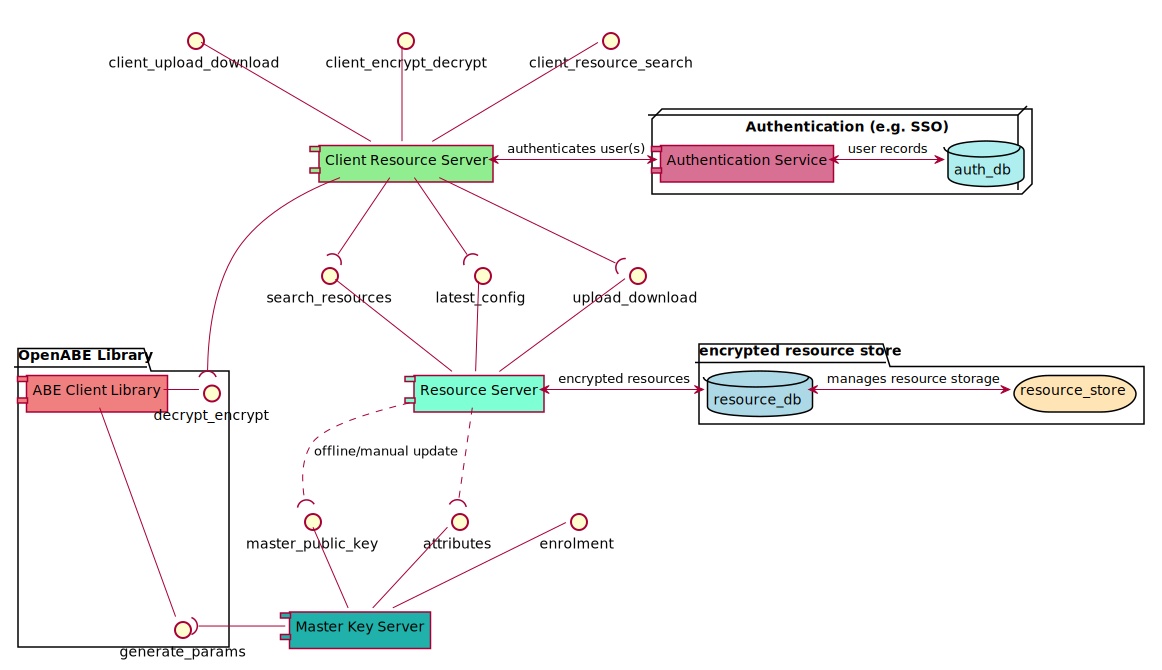
\includegraphics[width=\linewidth,keepaspectratio]{images/infrastructure/system_architecture_abbrv.pdf}

    \caption{
      \label{fig:sys_arch_abbrv}
      A condensed architecture diagram describing the system architecture of the \theResServer system. The \acrfull{mks} is in an offline state with access to a local copy of the \OpenABE library for provisioning the system \& generating user keys. The \acrfull{prs} is receiving offline updates from the \acrshort{mks}, managing a local database with resource metadata \& the associated resource storage and providing search, config and upload \& download interfaces for clients. The \acrfull{crs} has local access to an \OpenABE library for encryption \& decryption and access to an abstract Authentication Service (such as the university's SSO system). The \acrshort{crs} also implements the search, config and upload \& download interfaces provided by the \acrshort{prs} and provides its own upload \& download, encrypt \& decrypt and resource search interfaces for the user.
    }

\end{figure}


\section{Filename Searching}
\label{sec:design_file_search}

Users of the \theResServer system need to be able to identify resources they wish to download from the \acrfull{prs}. This may be trivial at first, since when there are only a few resources uploaded a user can easily browse a list to find the resources they need, however this quickly becomes infeasible as the \acrshort{prs} starts to store \textit{100s} of resources. Given the scale of the \acrfull{dcs}, this will become an issue quickly and so an alternative method of finding resources is required. Hence, we introduce a search utility for the \acrshort{prs}.
\vskip 0.5em
As described in \cref{subsec:design_resources}, the \acrshort{prs} stores the metadata of uploaded resources in a local database to maintain a complete unawareness of the contents of any resources. An advantage to this design, is that the database can be efficiently queried for complex searches over all resources uploaded, requiring no storage operations by the \acrshort{prs}'s \acrshort{os}\@. Additionally, in future the metadata stored for each resource can easily be expanded to meet the evolving needs of the \acrshort{dcs}.\\
The \acrfull{crs} implements the search utilities offered by the \acrshort{prs}, offering resource searching directly to the user, with the added benefit of obscuring resources that the user would not be able to decrypt. This is possible as the \acrshort{crs} is aware of the user's assigned attributes and the \acrshort{prs} records the policy of every resource in its database at upload-time, allowing for quick checks of a user's attributes against a resource's policy.
\vskip 0.5em
The \theResServer system is designed to implement a simple filename search utility with the possibility to extend searching to include any of the other metadata stored for resources in the future.\\
The filename searching itself is to operate in one of two methods, either by directly matching a slice of a filename and returning a sorted list of the most likely matches (e.g. the query \textit{``report.pdf''} would match the filename \texttt{one\_example\_report.pdf} but not \texttt{one\_example\_report.docx}) or in a fuzzy finder method which would more generally score the similarities between a query and all available filenames, returning a sorted list of the most likely matches (e.g. the query \textit{``pdf apple report four''} would match highly with the filenames \texttt{report\_hci\_four\_final.pdf} \& \texttt{rep\_on\_four\_apples.docx}).


\section{Summary}
\label{sec:design_summary}

We have presented the design of the \theResServer system, with a breakdown of the required software and the formal definition of a policy language, \thePolicyLang, that defines the types and syntax for \acrfull{abe} policies. We have also demonstrated use of \thePolicyLang to construct policies for 2 Case Studies \textit{(the remaining 4 Case Study policies are presented in Appendices \ref{appendix:case_study_0_policy}\textemdash\ref{appendix:case_study_4_policy})} and the process for users building new policies.

Finally, we discussed the user key design and system architecture for the \theResServer system, and described the design of a search utility for the \acrfull{prs} to enable users to discover resources.

%==================================================================================================================================
\chapter{Implementation}
\label{ch:implementation}

From the designs in \Cref{ch:design}, we present the implementation of the \theResServer system. With the \acrfull{mks}, \acrfull{prs} \& \acrfull{crs} implemented as web servers built from Python's Flask microframework using the \PyOpenABE library for \acrfull{abe}. The \acrshort{prs} implements filename searching and uses a local database for storing resource metadata.

\section{Python Web Servers}
\label{sec:impl_web_srvrs}

For the \theResServer system implementation, we require both a \acrfull{mks} and a \acrfull{prs} serving the requirements described in \cref{subsec:analysis_deployment_mks} and \cref{subsec:analysis_deployment_prs}. Both servers are to be implemented as web servers, allowing for simple \acrshort{html} \acrshort{gui}s to be built for user interactions. This allows for non-technical users to use the system without having to learn how to use \acrshort{cli} tools.\\
Additionally, since the \acrshort{mks} would have to integrate the \OpenABE library, it would need to be built with the C language or instead integrate with the \PyOpenABE library of bindings. Since building a web server in the C language was deemed to be an overly complex task for the length of time available to the project, and Python already offers web server frameworks (such as \href{http://flask.pocoo.org/}{Flask} \& \href{https://www.djangoproject.com/}{Django}), the project selected Python as the main language for implementation.\\
As a result, the \acrshort{mks} was built with the Python \href{http://flask.pocoo.org/}{Flask microframework} for its lightweight design and minimal feature set. Ultimately, relying on the fact that both web servers would only require very basic \acrshort{html} \acrshort{gui}s, which would not require the bulk of a Django project. Either framework would have provided the seamless integration of \PyOpenABE that was required for the \acrshort{mks}.
\vskip 0.5em
The \acrshort{prs} did not require integration with the \PyOpenABE library of bindings (as described in \cref{subsec:analysis_deployment_prs}) however did require a connection to a local database for storing metadata of resources. MongoDB was selected for this purpose (as explained in \cref{sec:impl_mongodb}) and Python offers the official \href{https://api.mongodb.com/python/current/}{PyMongo distribution} for this exact connection functionality.\\
Lastly, Python also offers a fuzzy string matcher, the \href{https://pypi.org/project/fuzzywuzzy/}{FuzzyWuzzy} package, to meet the filename searching needs detailed in \cref{sec:design_file_search}. This package combined with the built-in string matching of MongoDB (detailed in \cref{sec:impl_mongodb}) provides both methods required for filename searching.


\section{Creating the Client Server}
\label{sec:impl_client_srvr}

With both the \acrshort{mks} \& \acrshort{prs} built using Python's \href{http://flask.pocoo.org/}{Flask microframework}, when it came to building the \acrfull{crs}, the Flask microframework was selected again. This offered a level of code parity between the three products and offered the opportunity to reuse code from both the \acrshort{mks} \& \acrshort{prs} in the \acrfull{crs}, since it required integration with the \PyOpenABE library of bindings (like the \acrshort{prs}) as well as a PyMongo connection to a locally running MongoDB server (like the \acrshort{mks}).

The PyMongo connection was required to offer a pseudo-Authentication Service to the \acrshort{crs} for the project, in place of a real-world integration with a Single-Sign-On service. Whilst the \PyOpenABE library was required to offer encryption \& decryption services to the user, before uploading a resource and after downloading a resource.
\vskip 0.5em
The \acrshort{crs} was built to only run locally on a user's device and the pseudo-Authentication Service was built as a proof-of-concept as well. This means that the service is acknowledged as insecure, since a part of the service relies on storing the user's private user key in plaintext in the \textit{Users} table of the MongoDB database.

Importantly, this key \textbf{never} leaves the user's device during any encryption or decryption tasks, meaning the key is only vulnerable if the user's device \acrshort{os} is directly compromised. This means that in the event of the user's \acrshort{os} being compromised, their user key file would \textit{also} have been compromised anyway, and so the decision to have the user's key in plaintext within the database (\textit{for a proof-of-concept feature}) is not considered high risk. In a real-world deployment of the \theResServer system, this decision would not have to be made, as the system would be integrated with an external Authentication Service such as the university's Single-Sign-On system instead.

The \acrshort{crs} \textbf{does} implement secure password hashing with user accounts created for the pseudo-Authentication Service, using Python's package for \href{https://github.com/p-h-c/phc-winner-argon2}{argon2}, winner of the \href{https://password-hashing.net/}{Password Hashing Competition}, the pip package \href{https://pypi.org/project/argon2-cffi/}{\textit{argon2-cffi}}. This ensures that should a user set a password during registration that they then use with other services and their device becomes compromised, the \acrshort{crs} database cannot be abused to gain access to other services.


\section{Building with \OpenABE \& \PyOpenABE}
\label{sec:impl_openabe_libs}

\Cref{sec:bkgr_openabe} describes the \OpenABE library and its implementation of \acrfull{abe}, with \Cref{subsec:bkgr_pyopenabe} describing the \PyOpenABE bindings. The \OpenABE library is implemented with the C language and although the \PyOpenABE bindings are implemented in Python, they use the Cython language to bind Python functions to their C language equivalents (described in \Cref{subsec:bkgr_pyopenabe}).\\
As such, even though the \acrfull{mks} \& \acrfull{crs} are implemented with Python's Flask microframework and can directly use the \PyOpenABE library, the servers must also have a functioning C environment and the compiled \OpenABE library. The \theResServer system is designed for UNIX systems, meaning that the \acrshort{mks}, \acrshort{prs} \& \acrshort{crs} are all built for running on UNIX \acrshort{os} devices with C and Python environments installed and setup, this is an assumption for running the system.
\vskip 0.5em
Whilst installation instructions are provided individually by all the tools, libraries \& packages used by the \theResServer system, all installations rely on the environment being setup correctly. Throughout the project, this did not prove to be an issue for any of the software used, with the sole exception being the \OpenABE library. As such, a key requirement for running the \acrshort{mks} \& \acrshort{crs} services, is that the environment be prepared with a compiled \& tested version of the \OpenABE library before installation of any part of the \theResServer system (the \acrshort{prs} excluded, as it does not require \OpenABE or \PyOpenABE).\\
Further, the \PyOpenABE library of bindings must also be compiled \& tested before installation of either the \acrshort{mks} \& \acrshort{crs}, but the \PyOpenABE library appears to compile sufficiently as long as the \OpenABE library is properly configured.
\vskip 0.5em
As the \PyOpenABE library consists of bindings to the \OpenABE library, the values passed to \PyOpenABE functions (show in \cref{lst:python_encrypt} \& \cref{lst:python_decrypt}) are directly passed onto the underlying \OpenABE operations. Requiring that a policy for a resource to be encrypted with must be valid or a fatal error will be returned by \OpenABE.\\
The policy builder described in \Cref{sec:design_pol_build} provides this validation for users, by allowing a user to construct a new policy in \thePolicyLang and have it interpreted straight to a \PyOpenABE (and \OpenABE) compliant form. This interpretation is processed by \acrshort{html} \& Javascript in the user's browser and then sends the interpreted policy to the \acrshort{crs} Flask web server to be encrypted, with \PyOpenABE's \texttt{encrypt} function, as shown in \cref{lst:python_encrypt}.
\vskip 0.5em
When performing the decryption, the user provides an encrypted file that they wish to decrypt along with their user key, however in the case that the user has logged into the \acrshort{crs} with the pseudo-Authentication Service, the \acrshort{crs} will automatically retrieve the user's private key from the MongoDB database. The encrypted file and user key are then provided to \PyOpenABE's \texttt{decrypt} function, as shown in \cref{lst:python_decrypt}, which attempts to decrypt the file and if successful, the decrypted file is returned to the user.

\begin{lstlisting}[language=python, float, caption={Python code showing the encryption of a file using the \PyOpenABE library. Where \texttt{MASTER\_PUBLIC\_KEY} is the binary object representing the master public key, \texttt{file} is a binary stream of the file to be encrypted and \texttt{ct\_file} is a binary stream of the resulting encrypted file. The policy shown is the \PyOpenABE compliant policy as interpreted from the policy building described in \Cref{sec:design_pol_build} for Case Study \#1 (\cref{fig:case_study_policy_1}).}, label=lst:python_encrypt]
    policy = "username:jspringer or (staff and job_field:Research & Teaching) or (student and student_level = 2 and (enrolled_course:2001 and enrolled_course:2003 and enrolled_course:2007))"
    openabe, cpabe = create_cpabe_instance(MASTER_PUBLIC_KEY)
    try:
        ct_file = cpabe.encrypt(policy, file.read())
    except pyopenabe.PyOpenABEError as err:
        del openabe, cpabe
        flash(f"PyOpenABEError: {err}", 'danger')
        return render_template('encrypt.html', global_attrs=GLOBAL_ABE_ATTRS)
    del openabe, cpabe
\end{lstlisting}

\begin{lstlisting}[language=python, float, caption={Python code showing the decryption of an encrypted file using the \PyOpenABE library. Where \texttt{MASTER\_PUBLIC\_KEY} is the binary object representing the master public key, \texttt{key\_bytes} is a binary stream of the user's key, \texttt{username} is a string representing the user's username, \texttt{file\_bytes} is a binary stream of the encrypted file about to be decrypted and \texttt{dec\_file} is a binary stream of the resulting decrypted file.}, label=lst:python_decrypt]
    openabe, cpabe = create_cpabe_instance(MASTER_PUBLIC_KEY)
    cpabe.importUserKey(username, key_bytes)
    try:
        dec_file = cpabe.decrypt(username, file_bytes)
    except pyopenabe.PyOpenABEError as err:
        flash(f"Decryption of file failed: {err}", 'danger')
        dec_file = None
    del openabe, cpabe
\end{lstlisting}


\section{Using MongoDB for Data Storage}
\label{sec:impl_mongodb}

\Cref{sec:impl_web_srvrs} describes the \acrfull{prs} requirement that metadata for uploaded resources be stored in a local database, ensuring the \acrshort{prs} remains 


\section{Implementing a Fuzzy Finder for Filenames}
\label{sec:impl_fuzzy_finder}

\Cref{sec:design_file_search} describes the requirement of the \acrfull{prs} to offer a search utility to users and that it must offer two methods of searching. One method directly matches the query against slices of a filename and the other uses a fuzzy string matcher to generally score the similarities between a query and a filename. The second method is designed to help the user find resources they do not know much about and so may search with abstract query terms to find resources that might match.

\begin{lstlisting}[language=python, float, caption={Python code showing a PyMongo text search over the \textit{filename} text index.}, label=lst:pymongo_str_search]
    for resource in META_DB.find(
            {"$text": {"$search": search_term}},
            {"score": {"$meta": "textScore"}, "id": 1, "filename": 1}
    ).sort([("score", {"$meta": "textScore"})]).limit(search_limit):
        all_files.append({
            "id": str(resource["id"]),
            "filename": resource["filename"],
            "search_score": resource["score"]
        })
\end{lstlisting}

The first method is designed to be used by users specifically trying to find a file by a filename that they are able to at least partially recall. This method is much more efficient than the second method and can be implemented with direct use of MongoDB's \textit{text index} search functionality (\Cref{lst:pymongo_str_search}).

Where \texttt{search\_term} is a string representing the search query, \texttt{search\_limit} is an integer allowing the returned results to be limited and \texttt{all\_files} is a list that is filled with the resources collected by the search.

\begin{lstlisting}[language=python, float, caption={Python code showing a fuzzy string matching search over a collection of resources, using the \textit{fuzzywuzzy} package.}, label=lst:pymongo_fuzzy_search]
    from fuzzywuzzy import process
    ......
    searched_file_objs = process.extract(
            search_term, all_files, limit=fuzzy_limit)
        all_files = []
        for file in searched_file_objs:
            all_files.append(
                {"id": file[2], "filename": file[0], "search_score": file[1]})
\end{lstlisting}

The second method is more complex and requires the integration of a 3rd party fuzzy string matching package, Python's \href{https://pypi.org/project/fuzzywuzzy/}{FuzzyWuzzy}. First, the \acrshort{prs} must retrieve the metadata of the resources in the database before passing the retrieved metadata to the fuzzy string matcher. The \acrshort{prs} then extracts the fuzzy scores from the matcher and returns an ordered list of the highest scoring resource filenames. The code required to process the fuzzy matching is provided (\Cref{lst:pymongo_fuzzy_search}), however the MongoDB query that would precede this process is assumed to have taken place beforehand.

The process interface is first imported from \textit{fuzzywuzzy}, then the \texttt{extract()} function performs the matching and extracts the calculated scores for each resource. Where \texttt{search\_term} is a string representing the search query, \texttt{all\_files} is a list of all resources collected by a MongoDB find query and \texttt{fuzzy\_limit} is an integer allowing the returned results to be limited.


%==================================================================================================================================
\chapter{Evaluation}
\label{ch:evaluation}

Evaluation of the project is presented in the form of a risk assessment, verifying the security of the project and a discussion of the project achievements, with reference to the Case Studies designed in \Cref{sec:analysis_case_studies} that provide evidence that the system produced meets the needs of the users in the \acrfull{dcs}.

\section{Risk Assessment}
\label{sec:eval_risk_assess}

The \theResServer system is designed and implemented to be cryptographically secure with careful consideration of the security risks of deploying a public system. Where possible, steps have been taken to mitigate any risks to the system (see \Cref{sec:analysis_security} \& \Cref{sec:impl_web_srvrs}) and if not possible, the deployment or implementation has been designed to limit the system's exposure to risks (see \Cref{subsec:analysis_deployment_mks}).

Identifying the risks to the system was vital to creating a secure system that can be deployed publicly by the \acrfull{dcs} and ensured that the implementation was able to mitigate as many risks as possible. Identifying the risks to a system is not a simple task \citep{Gadd2003} and multiple organisations offer guidance on completing successful risk assessments without the common pitfalls \citep{HSE2014, EuropeanCommission2015}.
\vskip 0.5em
Internationally, the International Organisation of Standards (ISO) publishes standards that are applied across the world and as such its legislature is a more widely recognised body of work than that of the UK's Health and Safety Executive. As such this project decided to follow the ISO 27005:2008 \citep{ISO2008} for conducting a risk assessment on the \theResServer system.

Such a risk assessment requires an iterative process for identifying assets and their respective risks:
\begin{enumerate}
  \item
    Identify the assets in a system
  \item
    Identify the threats \& vulnerabilities
  \item
    Identify and estimate the risks to the assets
  \item
    Evaluate each risk
    \begin{itemize}
      \item[]
        If risk can be treated with a fix, jump to item \#5
      \item[]
        If risk can be treated through communication, jump to item \#6
      \item[]
        Risk cannot be treated, jump to item \#7
    \end{itemize}
  \item
    Carry out the fix and jump to item \#2
  \item
    Communicate the risk to users and jump to item \#2
  \item
    Risk cannot be treated, accept risk
  \item
    Continue to perform risk assessments, re-iterate for next assessment, jump to item \#1
\end{enumerate}

This process should be repeated for the life of a system, continually re-assessing the risks as the system evolves or expands, or as the environment changes.

\begin{table}[htp]
  \rowcolors{2}{}{gray!3}
  \begin{tabularx}{\linewidth}{lX}
    \textbf{Asset}            & \textbf{Description} \\
    Master Private Key file   &	Considered extremely high risk. MUST stay secret. \\
    Master Public Key file    &	Not dangerous, value is distributed as part of normal operation. \\
    Global Attributes file    &	As above, but potentially reveals information on the system. \\
    Server Secret (sessions)  &	Secret used to set up sessions with users, and generate CSRF tokens. \\
    Local web server files    &	Contains other config files, but also the key files. Needs protection. \\
    jinja2 plugin             &	Template plugin. Low risk, but external party provides software. \\
    flask plugin              &	Creates and runs the web server, some risk. By an external party. \\
    PyOpenABE bindings        &	Bindings for \OpenABE. High risk. Maintained by external party. \\
    cython lib/plugin         &	Binds Python to C. Interprets all bindings. So as above. \\
    Python3 lib               &	Python 3 environment. As above, lower risk, as globally reviewed. \\
    OpenABE C lib             &	\OpenABE library. High risk. Maintained by external party. \\
    C lib                     &	C environment. Low risk as global reviews \& slow to update as well. \\
    Firewall                  &	Firewall of host. Potential risk, but Key Server should be offline. \\
    User details              & Details a user has provided during the enrolment process. \\
    Generated User key        & Generated User keys. Held in memory, may be held in temp storage. \\
    Staff credentials         & Staff login credentials for the host machine OS. \\
    UNIX OS                   &	The UNIX OS of host. By external party so potential risk.
  \end{tabularx}
  \caption{Virtual assets for the \acrfull{mks}}
  \label{tab:assets_mk}
\end{table}

We present the virtual assets identified for the \acrfull{mks} in \Cref{tab:assets_mk} and refer to Appendix \ref{appendix:mks_assets} for the \acrshort{mks}'s physical assets. We further refer to the Appendices \ref{appendix:prs_assets} \& \ref{appendix:crs_assets} for the virtual \& physical assets of the \acrfull{prs} and \acrfull{crs}.

\begin{table}[htp]
  \begin{tabularx}{\linewidth}{|l|l|X|}
    \hline
    \rowcolor[HTML]{8497B0}
    \multicolumn{2}{|c|}{\cellcolor[HTML]{8497B0}\textbf{Threats}} & \multicolumn{1}{c|}{\cellcolor[HTML]{8497B0}} \\ \cline{1-2}
    \rowcolor[HTML]{FFD967}
    \multicolumn{1}{|c|}{\cellcolor[HTML]{FFD967}\textbf{Threat-Source}} & \multicolumn{1}{c|}{\cellcolor[HTML]{FFD967}\textbf{Threat-Actions}} & \multicolumn{1}{c|}{\multirow{-2}{*}{\cellcolor[HTML]{8497B0}\textbf{Vulnerabilities}}} \\ \hline
    \rowcolor[HTML]{A9D08E}
    \cellcolor[HTML]{F4B183} & Fire & Irreparable fire damage to equipment \\ \cline{2-3}
    \rowcolor[HTML]{A9D08E}
    \cellcolor[HTML]{F4B183} & Water Damage & Irreparable water damage to equipment \\ \cline{2-3}
    \rowcolor[HTML]{A9D08E}
    \cellcolor[HTML]{F4B183} & Pollution & Damage from pollution \\ \cline{2-3}
    \rowcolor[HTML]{A9D08E}
    \cellcolor[HTML]{F4B183} & Major Accident & Physical accident to equipment \\ \cline{2-3}
    \rowcolor[HTML]{A9D08E}
    \cellcolor[HTML]{F4B183} & \cellcolor[HTML]{A9D08E} & Lack of periodic replacement schemes \\ \cline{3-3}
    \rowcolor[HTML]{A9D08E}
    \cellcolor[HTML]{F4B183} & \cellcolor[HTML]{A9D08E} & Inadequate recruitment procedures (untrained/unskilled staff) \\ \cline{3-3}
    \rowcolor[HTML]{A9D08E}
    \cellcolor[HTML]{F4B183} & \multirow{-3}{*}{\cellcolor[HTML]{A9D08E}Destruction of Equipment or Media} & Inadequate or careless use of physical access control to buildings and rooms \\ \cline{2-3}
    \rowcolor[HTML]{A9D08E}
    \multirow{-8}{*}{\cellcolor[HTML]{F4B183}\textbf{Physical Damage}} & Dust, Corrosion, Freezing & Susceptibility to humidity, dust, soiling \\ \hline
  \end{tabularx}
  \caption{Sample of `physical damage' vulnerabilities from the ISO 27005:2008 standard.}
  \label{tab:example_threats_vulns}
\end{table}

With the assets identified, we present a sample of vulnerabilities from ISO 27005:2008 \citep{ISO2008}, the eight `Physical Damage' vulnerabilities, in \Cref{tab:example_threats_vulns}.

This represents just 5.1\% of the vulnerabilities assessed for the \theResServer system, with the full one hundred and fifty seven vulnerabilities in Appendix \ref{appendix:e_risk_assessment}. Each vulnerability is identified from a `Threat-Action' \textit{(e.g. Fire Damage, Water Damage)} with each `Threat-Action' being encompassed by a `Threat-Source' such as `Physical Damage'.

\begin{table}[htp]
  \begin{tabularx}{\linewidth}{Xllllll}
    \rowcolor[HTML]{9BC1E6}
    \multicolumn{1}{c}{\cellcolor[HTML]{8497B0}} & \multicolumn{3}{c}{\cellcolor[HTML]{9BC1E6}\textbf{Master Private Key file}} & \multicolumn{3}{c}{\cellcolor[HTML]{9BC1E6}\textbf{Master Public Key file}} \\
    \multicolumn{1}{c}{\multirow{-2}{*}{\cellcolor[HTML]{8497B0}\textbf{Vulnerabilities}}} & \cellcolor[HTML]{D87B79}\textbf{Impact} & \cellcolor[HTML]{C6E0B4}\textbf{Likelihood} & \cellcolor[HTML]{8EA9DB}\textbf{Risk} & \cellcolor[HTML]{D87B79}\textbf{Impact} & \cellcolor[HTML]{C6E0B4}\textbf{Likelihood} & \cellcolor[HTML]{8EA9DB}\textbf{Risk} \\
    \cellcolor[HTML]{A9D08E}Irreparable fire damage to equipment & 5 & 3 & \cellcolor[HTML]{FDBB7B}15 & 2 & 3 & \cellcolor[HTML]{A3C37C}6 \\
    \rowcolor[HTML]{EFEFEF}
    \cellcolor[HTML]{A9D08E}Irreparable water damage to equipment & 5 & 3 & \cellcolor[HTML]{FDBB7B}15 & 2 & 3 & \cellcolor[HTML]{A3C37C}6 \\
    \cellcolor[HTML]{A9D08E}Damage from pollution & 5 & 1 & \cellcolor[HTML]{96C27C}5 & 2 & 1 & \cellcolor[HTML]{6FBF7B}2 \\
    \rowcolor[HTML]{EFEFEF}
    \cellcolor[HTML]{A9D08E}Physical accident to equipment & 4 & 2 & \cellcolor[HTML]{BCC57C}8 & 2 & 2 & \cellcolor[HTML]{88C17B}4 \\
    \cellcolor[HTML]{A9D08E}Lack of periodic replacement schemes & 1 & 3 & \cellcolor[HTML]{7CC07B}3 & 1 & 3 & \cellcolor[HTML]{7CC07B}3 \\
    \rowcolor[HTML]{EFEFEF}
    \cellcolor[HTML]{A9D08E}Inadequate recruitment procedures (untrained/unskilled staff) & 3 & 4 & \cellcolor[HTML]{F0C97D}12 & 2 & 3 & \cellcolor[HTML]{A3C37C}6 \\
    \cellcolor[HTML]{A9D08E}Inadequate or careless use of physical access control to buildings and rooms & 5 & 2 & \cellcolor[HTML]{D6C77D}10 & 2 & 3 & \cellcolor[HTML]{A3C37C}6 \\
    \rowcolor[HTML]{EFEFEF}
    \cellcolor[HTML]{A9D08E}Susceptibility to humidity, dust, soiling & 3 & 2 & \cellcolor[HTML]{A3C37C}6 & 2 & 3 & \cellcolor[HTML]{A3C37C}6
  \end{tabularx}
  \caption{Sample of calculated impacts, likelihoods and risks for the `physical damage' vulnerabilities, regarding the public and private key files of the \acrfull{mks}.}
  \label{tab:example_vulns_risks}
\end{table}

Finally, we present \Cref{tab:example_vulns_risks}, a sample of calculated Impacts, Likelihoods and Risks for two of the assets identified in the \acrshort{mks}. For this purpose, the \textit{Master Private Key file} and \textit{Master Public Key file} assets were selected, and we again refer to \Cref{tab:example_threats_vulns} for the eight vulnerabilities that are sampled in \Cref{tab:example_vulns_risks}.

For each vulnerability, an asset was assigned a \texttt{Threat} score \textit{(1\textemdash5)} and a \texttt{Likelihood} score \textit{(1\textemdash5)}, where each scoring represented the threat from, or likelihood of, the vulnerability occurring. A final \texttt{Risk} was calculated for that asset as \texttt{Threat} * \texttt{Likelihood}, providing a \texttt{Risk} score of \textit{1\textemdash25}.
\vskip 0.5em
Appendix \ref{appendix:e_risk_assessment}, represents the full risk assessment with all calculations and insights, however, we summarise some of the results for the report.

\begin{table}[htp]
  \centering
  \rowcolors{2}{}{gray!3}
  \begin{tabular}{lllllll}
                    & \textbf{Asset Count}  & \textbf{Vuln. * Asset} & \textbf{High Risk} & \textbf{High \%} & \textbf{Low Risk} & \textbf{Low \%} \\
    \acrshort{mks}   &  30  & 4,710 & 12  &  0.25\% & 3,044  & 64.63\% \\
    \acrshort{prs}   &  19  & 2,983 & 1   &  0.03\% & 1,879  & 62.99\% \\
    \acrshort{crs}   &	32  & 5,024 & 6   &  0.12\% & 3,113  & 61.96\% \\
  \end{tabular}
  \caption{Analysis of Risk Assessment for \acrfull{mks}, \acrfull{prs} \& \acrfull{crs}}
  \label{tab:risk_assess_analysis}
\end{table}

As expected, the risk assessment identified the \acrfull{mks} as the highest \texttt{Risk} service with twelve high risk vulnerabilities. \Cref{tab:risk_assess_analysis} summarises the findings of the risk assessment for each server, where a high risk vulnerability is one with a \texttt{Risk} score greater than \textit{16/25} and a low risk vulnerability has a \texttt{Risk} score less than \textit{6/25}.

For the \acrshort{mks}, the following vulnerabilities were calculated as high risk with at least one asset:
\begin{enumerate}
  \item
    \textit{`Physical access to system not restricted appropriately'} \textemdash\ treated with the physical access restrictions described in \Cref{subsec:analysis_deployment_mks}.
  \item
    \textit{`System stores confidential information on storage'} \textemdash\ unavoidable, since the master private key must be stored somewhere, we accept this risk, but it can also be partially treated with physical access restrictions and storing the key on a \acrfull{hsm} as described by \citet{DBLP:conf/esas/TrichinaK04} and suggested by \citet{Akinyele2011}.
  \item
    \textit{`Escalated privileges grant full access to all information stored on system, including master signing key'} \textemdash\ as above, this is unavoidable and we must accept this risk but it can also be partially treated with physical access restrictions and storing the key on a \acrshort{hsm}.
  \item
    \textit{`Physical access to system grants full access to host data'} \textemdash\ treated with the physical access restrictions described in \Cref{subsec:analysis_deployment_mks}.
  \item
    \textit{`Admin staff could misplace user keys'} \textemdash\ cannot be fully treated, as human error will introduce some risk, however full training of staff should be a requirement for the granting of physical access to the \acrshort{mks} and would limit this risk.
  \item
    \textit{`Bugs in operating system could have drastic consequences on cryptographic integrity'} \textemdash\ the \acrshort{mks} host \acrshort{os} security is beyond the control of the project, we must accept that the \acrshort{os} could have bugs, we can partially treat by enforcing frequent security updates as they become available.
\end{enumerate}

For the \acrshort{prs}, the following vulnerability was calculated as high risk with at least one asset:
\begin{enumerate}
  \item
    \textit{`Escalated privileges grant full access to all information stored on system'} \textemdash\ the \acrshort{prs} does not store confidential information by design, however full access could enable a 3rd party to delete data from the local MongoDB database, potentially losing all stored metadata and would also allow the deletion of all store resources. This can be mitigated with frequent backups of the system, however even then, some data may be lost.
\end{enumerate}

For the \acrshort{crs}, the following vulnerabilities were calculated as high risk with at least one asset:
\begin{enumerate}
  \item
    \textit{`Physical access to system not restricted appropriately'} \textemdash\ the \acrshort{crs} runs on a user's local device and as such we have no control on physical access. If compromised, a user's private key could be stolen and resources could be decrypted with their key. Cannot be treated, we must accept this risk, and communicate the issues to users, explaining that it is their responsibility to protect their private key.
  \item
    \textit{`Physical access to system grants full access to host data'} \textemdash\ as above, this is unavoidable and we must accept this risk but we can communicate the risk to users, encouraging them to protect their devices with updates and strong passwords.
\end{enumerate}
\vskip 0.5em
We offer treatments where possible for the identified high risk vulnerabilities and otherwise acknowledge that we must accept and communicate the risk to users of the \theResServer system. The deployment of the \acrfull{mks} in an \textit{offline} state (as described in \Cref{subsec:analysis_deployment_mks} \& \Cref{sec:design_sys_arch}) mitigates the majority of the high risk vulnerabilities, as explained, and proves that the designed system is secure in both design and implementation.


\section{Achieved}
\label{sec:eval_achievements}


\section{Failed to Achieve}
\label{sec:eval_fail_achieve}


%==================================================================================================================================
\chapter{Conclusion}
\label{ch:conclusion}

The project produced a functioning resource server system, that is \textit{cryptographically secure} in implementation and designed for deployment in the \acrlong{dcs}. The \theResServer system offers a complete solution to users, providing a set of services to encrypt, decrypt, upload and download shared resources, within a simple \acrshort{gui}.

Security is key to the \theResServer system, and integration with an \acrfull{abe} library allows users to \textit{cryptographically} apply granular access policies to their resources, automatically enforcing end-to-end encryption in the process. Policies specify attributes that a user must possess to be able to decrypt the resources and proving possession requires a centrally signed private key.

The policies are created by the user using a custom policy building tool that adheres to a formal definition of the system's policy language, \thePolicyLang. The system consists of three base products, a \acrfull{mks} for signing user keys, a \acrfull{prs} for storing encrypted resources, and a local \acrfull{crs} provides the \acrshort{gui} for users.

The \theResServer system is proven to meet the needs of a resource server for the \acrfull{dcs} through six Case Studies simulating both common and complex scenarios for resource sharing in the \acrshort{dcs}. A further ISO 27005:2008-compliant risk assessment serves to verify the security of the system.

\section{Future Work}
\label{sec:concl_future_work}

Future work on the \theResServer system would focus on:
\begin{enumerate}
  \item
    \textbf{Authentication} \textemdash\ integration with a 3rd party Authentication Service, such as ActiveDirectory or the university's Single-Sign-On (SSO) system.
  \item
    \textbf{Policy Parsing} \textemdash\ functionality to parse a policy the user provides through a parser such as ANTLR, performing type checking on the policy.
  \item
    \textbf{Ciphertext Header} \textemdash\ implement a process for marking a ciphertext as ``created by the \theResServer system'', could add an identification header to ciphertext metadata.
  \item
    \textbf{Selective Uploads} \textemdash\ only allow uploading of resources that were encrypted by the \theResServer system and thus have an identification header in the ciphertext metadata.
  \item
    \textbf{Attribute Collecting} \textemdash\ interface with systems such as the Student Centre/MyCampus and the HR/Payroll system to automatically collect a new user's attributes, reducing risk of human error.
  \item
    \textbf{Backup System} \textemdash\ implement a secure backup system for the \acrfull{prs}, protecting against loss of data.
\end{enumerate}


%==================================================================================================================================
%
%
%==================================================================================================================================
%  APPENDICES

\begin{appendices}

\chapter{Appendices}

\section{Appendix A - Deployment Roles \& Users}
\label{appendix:roles_users}

Mind Map representing the identified user roles of the Department of Computing Science in red to the left and the identified users in blue to the right.

\includegraphics[width=\linewidth]{appendices/mind_maps/ABE_Users_slides_Oct26.pdf}

\section{Appendix B - Enrolment Diagram for Staff User}
\label{appendix:enrolment_diagram}

\begin{figure}
    \centering
    \includegraphics[width=\linewidth,keepaspectratio]{appendices/diagrams/flow_of_info/enrollment_stu_sequence.pdf}

    \caption{A sequence diagram demonstrating the enrolment process for a student. The student can be seen requesting a user key \#1 (and providing their student ID) from the DCS Teaching Assitant, whom verifies the student's identity and then retrieves their details \#2 from the Student Centre (or MyCampus) system. The Teaching Assistant then processes the returned attributes \#5 for the Master Key Server, and then requests a new key \#6 by providing the student's attributes. The Master Key Server can be seen processing \#7 and then returning the newly generated key \#8 to the Teaching Assistant, whom finally provides the key to the student.}
    
\end{figure}

\end{appendices}


%==================================================================================================================================
%   BIBLIOGRAPHY

% The bibliography style is abbrvnat
% The bibliography always appears last, after the appendices.

\bibliographystyle{abbrvnat}

\bibliography{l4proj}

\newpage

\printnoidxglossaries

\end{document}
